\documentclass[11pt, a4paper]{article}
%\usepackage{proj1}
\usepackage{natbib}
\usepackage{fancyhdr}  
\usepackage{subcaption}
\usepackage{caption}
\usepackage{graphicx}
\linespread{1.25} 
\setlength{\parindent}{0cm}
\graphicspath{{Images/}}
\usepackage{hyperref}
\usepackage{amsmath}
\usepackage{amsfonts}
\usepackage{amssymb}
\usepackage{amsthm}
\usepackage{numprint}
\usepackage{mathtools}
\usepackage{commath}
\usepackage{bbm}

%\usepackage[sc,osf]{mathpazo}
\usepackage{subcaption}
\usepackage[a4paper, top=1in, left=1.0in, right=1.0in, bottom=1in, includehead, includefoot]{geometry} %Usually have top as 1in

\usepackage{listings}
\usepackage{color} %red, green, blue, yellow, cyan, magenta, black, white
\definecolor{mygreen}{RGB}{28,172,0} % color values Red, Green, Blue
\definecolor{mylilas}{RGB}{170,55,241}


\hypersetup{colorlinks,linkcolor={black},citecolor={blue},urlcolor={black}}
\usepackage{color}
\urlstyle{same}


\theoremstyle{definition}
\newtheorem{definition}{Definition}[section]

%\newcommand{\Sta}{\rho}
\newcommand{\Adj}{p}
\newcommand{\adj}{q}
%\newcommand{\Con}{u}
\newcommand{\Sta}{\rho}
\newcommand{\Stav}{\mathbf{v}}
\newcommand{\Adja}{\mathbf{p}}
\newcommand{\Adjb}{q}
\newcommand{\Adjc}{{q}_{\partial \Omega}}
\newcommand{\Con}{\mathbf{f}}
\newcommand{\nor}{\mathbf{n}}



\title{Report, PhD Year 2}
\author{Jonna C. Roden\\ \\Supervision by Dr Ben Goddard and Dr John Pearson\\ \\ \vspace{0.5cm} MIGSAA}
\date{\today}


\pagenumbering{gobble}
\begin{document}
	\lstset{language=Matlab,%
		%basicstyle=\color{red},
		breaklines=true,%
		morekeywords={matlab2tikz},
		keywordstyle=\color{blue},%
		morekeywords=[2]{1}, keywordstyle=[2]{\color{black}},
		identifierstyle=\color{black},%
		stringstyle=\color{mylilas},
		commentstyle=\color{mygreen},%
		showstringspaces=false,%without this there will be a symbol in the places where there is a space
		numbers=left,%
		numberstyle={\tiny \color{black}},% size of the numbers
		numbersep=9pt, % this defines how far the numbers are from the text
		emph=[1]{for,end,break},emphstyle=[1]\color{blue}, %some words to emphasise
		%emph=[2]{word1,word2}, emphstyle=[2]{style},    
		basicstyle=\footnotesize\ttfamily,
	}
	
	\maketitle
%	\begin{abstract}
%		Sum up the below here!
%		
%	\end{abstract}
%	
	\newpage
%	\section*{Acknowledgements}
%	+Acknowledge People Here+
%	\newpage
	\pagenumbering{Roman} 
	\tableofcontents
	%\newpage
	%\listoffigures
	%\listoftables
	\newpage
	\pagenumbering{arabic} % Switch to normal numbers
	%\pagestyle{fancy}
















\section{Introduction}
In this report, an overview is given on the work that has been carried out during the past year. First, a literature review on related work in mean field optimal control is provided. Then, different equations are discussed, which model particle dynamics and serve as PDE constraints in the considered optimal control problems. In particular, the we consider PDEs which include inertial effects and their high friction limit, the so called overdamped equations. We then derive optimality conditions for PDE-constrained optimizaion problems involving both of these cases. Most of the work on the numerical method has been done using the overdamped limit as PDE constraint. 
The main focus of this year's work was the implementation of a fast and accurate optimization solver for different PDE-constrained optimization problems. Building on the extended project report, different optimization methods are briefly presented and compared. The fastest solver is then validated and applied to various test problems.
Finally, an outlook is given on future work. In the appendix it is detailed which other activities outside the PhD project have been completed and an overview on future participation in various activities is provided.


\section{Literature Review on Mean Field Optimal Control}

While mean-field games were first introduced by Lasry and Lions, \cite{LASRY2006619}, \cite{LASRY2006679},\cite{LASRY4} and \cite{Lasry2007}, and independently by Huang, Caines and Malham\'e,  \cite{Huang1}, under the name Nash certainty equivalence, the optimal control side of this class of problems is quite a new area of research. The main difficulty in the optimal control of mean-field equations is a non-linear, non-local particle interaction term. Therefore, standard results in optimal control theory cannot readily be applied, and new approaches have to be developed to address theoretical and numerical challenges.
\\
\\
There are two types of models that recent work has focussed on. The most popular model is a deterministic microscopic model, which is a generalization of the well-known Cucker-Smale model, see \cite{CuckerSmale1}, \cite{CuckerSmale2}. In the mean-field limit, a Vlasov-type PDE arises. For control problems involving this class of models, the work by Fornasier et al. provides a range of theoretical results on the convergence of the microscopic optimal control problem to a corresponding macroscopic problem, using methods of optimal transport and a $\Gamma$-limit argument, proving existence of optimal controls in the mean-field setting, see \cite{Fornasier_2014},
\cite{Fornasier_2014no2}
and \cite{fornasier_lisini_orrieri_savare_2019}. The work focusses on sparse control strategies, where one or more agents influence a larger crowd.
Additional work on sparse control strategies can be found in \cite{piccoli2014no1}, as well as in the review paper \cite{Fornasier_20161no1}.
In \cite{burger2019meanfield}, an alternative method, an $L_2$ calculus, is developed, and convergence results are proved. The control in this work is applied through the interaction term. 
\\
Numerical advances have been made in \cite{burger2019instantaneous} and \cite{burger2016controlling}, where sparse and other control strategies through the external agents are considered. In both papers a Strang-Splitting scheme, \cite{ChengC.Z1976Tiot}, is applied to solve the optimal control problem. The numerical results verify the convergence of the microscopic control problem to its mean-field limit.
Furthermore, in \cite{albi2016selective}, different selective control strategies are considered, and an iterative numerical method is chosen, where the interaction term is approximated stochastically.
\\
\\
Fewer work has been done on the optimal control of the Fokker-Planck PDE, which arises as the mean-field limit of a stochastic microscopic model. Some theoretical results on this model are published. In \cite{albi2016mean}, the existence of optimal controls for microscopic and macroscopic versions of a class of problems are proved and a rigorous derivation of first-order optimality conditions is given. 
Following this, \cite{carrillo2019mean} discusses the existence and regularity of an optimal control problem of this type on periodic domains, including the well-posedness of the Fokker-Planck equation. In \cite{Pinnau_2017} and  \cite{carrillo2018no1}, the convergence of the microscopic optimal control problem to its mean-field limit is proved.
Numerical results on the model include those presented in \cite{Pinnau_2017}, where a Strang-Splitting scheme, \cite{gilbertstrang1}, is applied, and in which convergence to the mean field optimal control problem is shown numerically. Furthermore, in \cite{albi2016mean}, an optimal control hierarchy, including instantaneous and Boltzmann-type controls, is proposed. The mean-field first-order optimality system in \cite{albi2016mean} is solved using a Chang-Cooper scheme for the forward equation, finite differences for the adjoint equation, while approximating the integrals using a Monte-Carlo scheme. This is coupled by a sweeping algorithm, where updates are made through the gradient equation.
Some numerical results on a porous media version of the Fokker-Planck equation are presented in \cite{carrillo2018no1}. In \cite{Albi_2014no1} and \cite{albi2014kinetic}, steady state solutions to a Fokker-Planck-type PDE are considered, however, the main focus  are Boltzmann-type approaches to solving the optimal control problem.
\\
\\
The most common control types in the literature are flow control, e.g. \cite{albi2016mean}, control through the interaction term, e.g. \cite{Pinnau_2017}, as well as control through external agents, e.g. \cite{Fornasier_2014no2}. 
Most papers do not consider boundary conditions, because it is assumed that the particle distribution is of compact support, see \cite{burger2019meanfield}, \cite{fornasier_lisini_orrieri_savare_2019} or \cite{burger2016controlling}. No-flux boundary conditions, which are of high relevance in applications, are not often found in the literature, but are considered in \cite{albi2016mean} and \cite{carrillo2018no1}.
Our work considers the mean-field equation of Fokker-Planck type, flow-type control or control through a force term and no-flux or Dirichlet boundary conditions, in order to address a broad range of test problems and real world applications. 
\\
\\
As described above, some numerical methods have been developed for solving optimal control problems involving non-local, non-linear PDEs. Most of these papers however focus on other methods and use the mean-field optimal control as verification tool, see \cite{Pinnau_2017}, \cite{albi2016mean}. It takes large computational effort to solve these problems, which increases with dimensionality, see \cite{burger2019instantaneous}, \cite{burger2016controlling}. 
We are proposing a new numerical framework for PDE-constrained optimization applied to multiscale particle dynamics, where a fixed point algorithm is implemented to solve the first-order optimality system. This update scheme is inspired by the sweeping algorithm in \cite{albi2016mean}, and equivalent to the gradient descent method in \cite{Burger1}. The algorithm is coupled with pseudospectral methods, used to discretize space and time domains. This composition of methods offers an efficient and accurate solver for the class of problems discussed. To our knowledge, it is the first time that pseudospectral methods are used in the context of optimal control problems.










\section{Discussion of Relevant Equations and their Optimality Conditions}
\subsection{The Studied Equations}
This section is concerned with discussing different equations that have been studied in the past year and the derivation of the optimality conditions of optimal control problems with constrains involving these equations. The discussion of the forward equations and their connections is heavily based on \cite{Archer1}.

The most general equations considered, describing particle dynamics on a continuum level, are the so-called inertial equations. These are derived in \cite{Archer1}, by A.J.Archer, from the corresponding microscopic dynamics. The derivation includes taking momentum moments and making two modelling assumptions. The first assumption is that the contributions of particle interactions in the dynamic equations can be approximated by the interactions in equilibrium. The second assumption is a 'local-equilibrium' assumption, assuming that locally the velocity is normally distributed. This assumption is violated when steep velocity gradients arise, which will be discussed below.

The inertial equations are most generally formulated as:
\begin{align*}
	&\frac{\partial \Stav}{\partial t} + \Stav \cdot \nabla \Stav + \gamma \Stav = - \frac{1}{m} \nabla \frac{\delta \mathcal{F}[\Sta]}{\delta \Sta}\\
	&\frac{\partial \Sta}{\partial t} + \nabla \cdot (\Sta \Stav) =0
\end{align*}
This system of equations describes the evolution of a velocity field $\Stav$ and of the one-body particle density $\Sta$, which depends on the velocity field.
The velocity in the system is influenced by inertial effects, with friction coefficient $\gamma$, and by different forces, expressed in terms of the free energy $\mathcal{F}$ of the system.
In the following we choose $\mathcal{F}$ to be defined as:
\begin{align*}
\mathcal{F}[\Sta]=\int_\Omega  \bigg( V_{ext}\Sta + \Sta (\log \Sta -1) +  \frac{1}{2}\int_\Omega \Sta(r) \Sta(r')V_2(|r-r'|)dr' \bigg) dr.
\end{align*}
Taking the appropriate derivatives gives:
\begin{align*}
 \nabla \frac{\delta \mathcal{F}[\Sta]}{\delta \Sta} = \nabla V_{ext} + \nabla \ln \Sta + \int_\Omega \Sta(r') \nabla V_2(|r-r'|)dr',
\end{align*}
where $\nabla V_2$ is the force describing the particle interactions. However, in the derivation of corresponding optimality conditions, we instead consider a general interaction kernel $\mathbf{K}(r,r')$.
\\
Further to this general model, we introduce three more terms for modelling purposes. Two vector fields, $\mathbf{w}$ and $\Con$, are included in the velocity equation, which act as background flow fields in the problem. If these are conservative, they can be incorporated in the definition of $\nabla V_{ext}$. The term $\mathbf{w}$ will act as the flow control in the optimal control problem.
The final term that is added is a smoothing term for the velocity. This is to avoid steep velocity gradients, which are numerically challenging and violate the modelling assumptions outlined in \cite{Archer1}. Since steep velocity gradients are more prevalent in inertial systems, which have a small friction coefficient $\gamma$, the introduction of this additional term is standard practice, see \cite{Archer1} (+1 more?).
Including these terms leads to the model equations considered in this report:
\begin{align}
\label{eqn:INeqns1}
\frac{\partial \Stav}{\partial t} &+ (\Stav \cdot \nabla)\Stav + \gamma \Stav=\eta \nabla^2 \Stav  -\frac{1}{m}\Con +\frac{1}{m}\mathbf{w} - \frac{1}{m}\nabla \frac{\delta \mathcal{F}[\Sta]}{\delta \Sta}\\
\frac{\partial \Sta}{\partial t} &+ \nabla \cdot (\Sta \Stav)=0 \notag
\end{align}
The high friction limit of the inertial equations can be taken to derive the so-called overdamped eqation, see \cite{Archer1}. This is a numerically easier problem, which only involves the variable $\rho$, and not $\Stav$ and is therefore a good starting point when developing a new numerical algorithm for their optimal control. 
The overdamped eqaution is derived by assuming that for large $\gamma$ the material derivative of $\Sta$, $\frac{D \Sta}{D t} \coloneqq  \frac{\partial \Stav}{\partial t} + (\Stav \cdot \nabla)\Stav$ is zero.
Then Equations (\ref{eqn:INeqns1}) reduce to:
 \begin{align*}
&\gamma \Stav=\eta \nabla^2 \Stav  -\frac{1}{m}\Con +\frac{1}{m}\mathbf{w} - \frac{1}{m}\nabla \frac{\delta \mathcal{F}[\Sta]}{\delta \Sta}\\
 &\frac{\partial \Sta}{\partial t} + \nabla \cdot (\Sta \Stav)=0 \notag.
 \end{align*}
Then, $\Stav$ can be substituted in the evolution equation for $\rho$, and the smoothing term for $\Stav$ can be neglected, since the high friction limit is taken and the reason for its introduction hence vanishes. The overdamped equation is:
  \begin{align*}
 &\frac{\partial \Sta}{\partial t} -\frac{1}{m \gamma}\nabla \cdot (\Sta\Con) +\frac{1}{m \gamma} \nabla \cdot (\Sta \mathbf{w}) - \frac{1}{m \gamma}\nabla \cdot \bigg(\Sta\nabla \frac{\delta \mathcal{F}[\Sta]}{\delta \Sta}\bigg)=0 \notag.
 \end{align*}
 In particular, substituting the choice of free energy introduced above, and using that $\nabla \rho = \rho\nabla \ln \rho$, we get:
\begin{align*}
\frac{\partial \Sta}{\partial t} &= \frac{1}{m \gamma}\nabla \cdot (\Sta\Con) -\frac{1}{m \gamma} \nabla \cdot (\Sta \mathbf{w})  + \frac{1}{m \gamma}\nabla \cdot (\rho\nabla V_{ext}) + \frac{1}{m \gamma}\nabla \cdot (\nabla \rho) \\
&+\frac{1}{m \gamma}\nabla \cdot \int_\Omega \Sta(r)\Sta(r') \nabla V_2(|r-r'|)dr'\notag.
\end{align*}
The overdamped equation that is considered in this report, is found by rescaling time: $t = \tilde t \gamma m$. This causes the constants to cancel, and implies that comparison between (\ref{eqn:INeqns1}) and (\ref{eqn:ADeqn1}) need to be made on the two different time scales.
The resulting equation is:
\begin{align*}
\label{eqn:ADeqn1}
\frac{\partial \Sta}{\partial \tilde t} &= \nabla \cdot (\Sta\Con) - \nabla \cdot (\Sta \mathbf{w})  + \nabla \cdot (\rho\nabla V_{ext}) + \nabla \cdot (\nabla \rho) \\
&+\nabla \cdot \int_\Omega \Sta(r)\Sta(r') \nabla V_2(|r-r'|)dr'.
\end{align*}
\subsection{Optimality Conditions for the Inertial Eqations}



\subsubsection{PDE-Constrained Optimization Problem}
The domain is $\Sigma=\Omega \times [0,T]$. There are two state variables, the particle density $\Sta$ and the velocity $\Stav$. The control is a background flow term $\mathbf{w}$. 
\begin{align*}
&\min_{\Sta,\Stav,\mathbf{w} } \quad \frac{1}{2}||\Sta - \hat \Sta||_{L_2(\Sigma)}^2  +\frac{\beta}{2}||\mathbf{w}||_{L_2(\Sigma)}^2\\
&\text{subject to:}\\
&m \Sta \frac{\partial \Stav}{\partial t}= - m \Sta (\Stav \cdot \nabla)\Stav -\Sta \nabla V_{ext} -\Sta \Con -\Sta \mathbf{w} - \nabla \Sta - m\gamma \Sta \Stav + \eta \rho \nabla^2 \Stav \\
& \quad \quad -\int_\Omega \rho(r) \rho(r') \nabla V_2(|r-r'|)dr' \\
&\frac{\partial \Sta}{\partial t} + \nabla \cdot (\Sta \Stav)=0 \qquad\qquad \qquad\qquad\qquad\quad \quad\quad\qquad \qquad\qquad \qquad\qquad\qquad\quad \qquad\qquad\qquad\quad\ \ \text{in} \quad \Sigma\\
\\
&\Sta \Stav \cdot \mathbf{n} =0\qquad\qquad \qquad\qquad\qquad\qquad\qquad\qquad\qquad \qquad\qquad \qquad\qquad\qquad \qquad\qquad\qquad\quad \qquad \text{on} \quad \partial  \Sigma\\
& \Sta(r,0)=\Sta_0\\
& \Stav(r,0)=\Stav_0.
\end{align*}
Here, we have (I am not sure how to/ if to include $\rho \Con$, $\rho \mathbf{w}$.):
\begin{align*}
\mathcal{F}[\Sta]=\int_\Omega  \bigg( V_{ext}\Sta + \Sta (\log \Sta -1) +  \int_\Omega \Sta(r) \Sta(r')V_2(|r-r'|)dr' \bigg) dr.
\end{align*}

Then:
\begin{align*}
\rho \nabla \frac{\delta \mathcal{F}[\Sta]}{\delta \Sta} = \Sta \nabla V_{ext} + \nabla \Sta + \int_\Omega \Sta(r) \Sta(r') \nabla V_2(|r-r'|)dr',
\end{align*}
which matches Equation $(29)$ in Archer's paper.
\subsubsection*{The Lagrangian}
The Lagrangian for the above problem is:
\begin{align*}
&\mathcal{L}(\Sta,\Stav,\mathbf{w},\Adja,\Adjb,\Adjc) = \int_0^T \int_\Omega  \frac{1}{2}(\Sta - \hat \Sta)^2 drdt  +\int_0^T \int_\Omega  \frac{\beta}{2}\mathbf{w}^2 drdt\\
&+ \int_0^T \int_\Omega (m \Sta \frac{\partial \Stav}{\partial t} + m \Sta (\Stav \cdot \nabla)\Stav + \Sta \nabla V_{ext} + \Sta \Con + \Sta \mathbf{w} + \nabla \Sta + m\gamma \Sta \Stav  - \rho \eta \nabla^2 \Stav\\
&+\int_\Omega \rho(r) \rho(r') \nabla V_2(|r-r'|)dr') \cdot \Adja dr dt\\
& + \int_0^T \int_\Omega (\frac{\partial \Sta}{\partial t} + \nabla \cdot (\Sta \Stav)) \Adjb dr dt\\ 
& +\int_0^T \int_{\partial\Omega} \Sta \Stav \cdot \mathbf{n} \Adjc dr dt,
\end{align*}
where $\Adja$, $\Adjb$ and $\Adjc$ are Lagrange multipliers associated with the PDE for $\Stav$, the PDE for $\Sta$ and the boundary condition, respectively.
\subsubsection{Adjoint Equation 1}

The derivative of $\mathcal{L}$ with respect to $\Sta$ in some direction $h$ is, where ${h} \in C_0^\infty(\Sigma) $:
\begin{align*}
&\mathcal{L}_\Sta(\Sta,\Stav,\mathbf{w},\Adja,\Adjb,\Adjc)h = \int_0^T \int_\Omega  (\Sta - \hat \Sta)h drdt \\
&+ \int_0^T \int_\Omega (m h \frac{\partial \Stav}{\partial t}\cdot \Adja + m h( (\Stav \cdot \nabla)\Stav )\cdot \Adja+ h\nabla V_{ext}\cdot \Adja + h \Con \cdot  \Adja + h \mathbf{w} \cdot \Adja + \nabla h\cdot \Adja - \eta h \nabla^2 \Stav \cdot \Adja)  dr dt\\
&+ \int_0^T \int_\Omega (m\gamma h \Stav +\int_\Omega h(r) \rho(r') \nabla V_2(|r-r'|)dr'+\int_\Omega \rho(r) h(r') \nabla V_2(|r-r'|)dr') \cdot \Adja dr dt\\
& + \int_0^T \int_\Omega (\Adjb\frac{\partial h}{\partial t} + \Adjb\nabla \cdot (h \Stav))  dr dt +\int_0^T \int_{\partial\Omega} \Adjc h\Stav \cdot \mathbf{n}  dr dt,
\end{align*}
where the product rule is used to take the derivative of the interaction term. Looking at different integral terms individually:
\begin{align*}
I_1= \int_0^T \int_\Omega \nabla h\cdot \Adja dr dt = \int_0^T \int_{\partial \Omega} h \Adja \cdot \mathbf{n} dr dt - \int_0^T \int_{\Omega} \nabla\cdot \Adja h dr dt
\end{align*}
 
\begin{align*}
I_2 = \int_0^T \int_\Omega \Adjb\frac{\partial h}{\partial t} dr dt = \int_\Omega h(T) \Adjb(T) dr dt - \int_0^T \int_\Omega  \frac{\partial \Adjb}{\partial t}h dr dt
\end{align*}
Note that ${h}(r,0)=0$, (in order to satisfy the condition for all admissible ${h}$) and so the initial condition vanishes from the above expression.
\begin{align*}
I_3= \int_0^T \int_\Omega \Adjb\nabla \cdot (h \Stav) dr dt = \int_0^T \int_{\partial \Omega} \Adjb \Stav \cdot \mathbf{n} h dr dt - \int_0^T \int_\Omega \nabla \Adjb \cdot \Stav h dr dt.
\end{align*}
Furthermore, we have:
\begin{align*}
I_{2B}&= \int_0^T \int_\Omega \bigg(\int_\Omega \rho(r) h(r') \nabla V_2(|r-r'|)dr'\bigg) \cdot \Adja(r) drdt\\
&=\int_0^T \int_\Omega \int_\Omega \rho(r) h(r') \nabla V_2(|r-r'|) \cdot \Adja(r) drdr'dt,
\end{align*}
swapping the order of integration. Then we have:
\begin{align*}
I_{2B}&= \int_0^T \int_\Omega  h(r')\bigg(\int_\Omega  \rho(r)\nabla V_2(|r-r'|) \cdot \Adja(r) dr \bigg)dr'dt,
\end{align*}
and relabelling $r \to r'$ and $r' \to r$ gives:
\begin{align*}
I_{2B}&= -\int_0^T \int_\Omega  h(r)\bigg(\int_\Omega  \rho(r')\nabla V_2(|r-r'|) \cdot \Adja(r') dr' \bigg)drdt.
\end{align*}
The introduction of the minus sign is due to the relationship $\nabla_r V_2(|r - r'|) = \nabla_{r'} V_2(|r' - r|)$.  (++ Check correct location of comment)+++
Replacing $I_1, I_2, I_{2B}$ and $I_3$ in the derivative gives:
\begin{align*}
&\mathcal{L}_\Sta(\Sta,\Stav,\mathbf{w},\Adja,\Adjb,\Adjc)h = \int_\Omega h(T) \Adjb(T) dr dt  \\
&+ \int_0^T \int_\Omega \bigg( (\Sta - \hat \Sta) +m  \frac{\partial \Stav}{\partial t}\cdot \Adja + m  ((\Stav \cdot \nabla)\Stav )\cdot \Adja+ \nabla V_{ext}\cdot \Adja + \Con \cdot \Adja + \mathbf{w} \cdot \Adja \\
&- \eta \nabla^2 \Stav \cdot \Adja -\nabla\cdot \Adja  - \ \nabla \Adjb \cdot \Stav  -  \frac{\partial \Adjb}{\partial t} + m \gamma \Stav \cdot \Adja\bigg) h dr dt \\
&+ \int_0^T \int_\Omega  \bigg(\int_\Omega  \rho(r')(\Adja(r) - \Adja(r')) \cdot\nabla V_2(|r-r'|)   dr'  \bigg)hdr dt\\
&+\int_0^T \int_{\partial \Omega} ( \Adja \cdot \mathbf{n}  +  \Adjb \Stav \cdot \mathbf{n}   +\Adjc \Stav \cdot \mathbf{n})h  dr dt
\end{align*}
Setting $\mathcal{L}_\Sta(\Sta,\Stav,\Con,\Adja,\Adjb,\Adjc)h=0$, and restricting the admissible set of choices of $h$ to:
\begin{align*}
h&=0 \quad \text{on} \quad \partial \Sigma\\
h(T)&=0.
\end{align*}
Then the derivative becomes:
\begin{align*}
 &\int_0^T \int_\Omega \bigg( (\Sta - \hat \Sta) +m  \frac{\partial \Stav}{\partial t}\cdot \Adja + m  ((\Stav \cdot \nabla)\Stav )\cdot \Adja+ \nabla V_{ext}\cdot \Adja + \Con \cdot \Adja + \mathbf{w} \cdot \Adja \\
 &- \eta \nabla^2 \Stav \cdot \Adja  -\nabla\cdot \Adja  - \ \nabla \Adjb \cdot \Stav  -  \frac{\partial \Adjb}{\partial t} +m \gamma \Stav \cdot \Adja \bigg) h dr dt \\
 &+ \int_0^T \int_\Omega \bigg(  \int_\Omega  \rho(r')(\Adja(r) - \Adja(r')) \cdot\nabla V_2(|r-r'|)   dr'  \bigg)hdr dt\\
 &=0.
\end{align*}
Since this has to hold for all $h \in C_0^\infty(\Sigma)$ and $C_0^\infty(\Sigma)$ is dense in $L_2(\Sigma)$, the first adjoint equation is derived as:
\begin{align}
& \frac{\partial \Adjb}{\partial t} = (\Sta - \hat \Sta) +m  \frac{\partial \Stav}{\partial t}\cdot \Adja + m ( (\Stav \cdot \nabla)\Stav) \cdot \Adja+ \nabla V_{ext}\cdot \Adja + \Con \cdot \Adja + \mathbf{w} \cdot \Adja  - \eta \nabla^2 \Stav \cdot \Adja \\
&-\nabla\cdot \Adja  -  \nabla \Adjb \cdot \Stav + m \gamma \Stav \cdot \Adja + \int_\Omega  \rho(r')( \Adja(r) - \Adja(r') ) \cdot\nabla V_2(|r-r'|)   dr' \qquad \text{in} \quad \Sigma \notag
\end{align}
Then, relaxing the conditions on $h$, such that $h(T) \neq 0$ is a permissible choice, gives:
\begin{align*}
\int_\Omega h(T) \Adjb(T) dr dt=0,
\end{align*}
and by the same density argument as above, this gives the final time condition for $\Adjb$:
\begin{align*}
\Adjb(T) = {0} .
\end{align*}
Finally, allowing $h \neq 0 \quad \text{on} \quad \partial \Sigma$ result in:
\begin{align*}
\int_0^T \int_{\partial \Omega} ( \Adja \cdot \mathbf{n}  +  \Adjb \Stav \cdot \mathbf{n}   +\Adjc \Stav \cdot \mathbf{n})h  dr dt=0,
\end{align*}
and again by a density argument:
\begin{align*}
 \Adja \cdot \mathbf{n}  +  \Adjb \Stav \cdot \mathbf{n}   +\Adjc \Stav \cdot \mathbf{n} = 0\qquad \text{on} \quad \partial \Sigma
\end{align*}
Since $\Stav \cdot \mathbf{n} =0$ on $ \partial \Sigma$, the boundary condition reduces to:
\begin{align*}
\Adja \cdot \mathbf{n} = 0 \qquad \text{on} \quad \partial \Sigma.
\end{align*}
Therefore, the first adjoint equation of this problem is:
\begin{align*}
& \frac{\partial \Adjb}{\partial t} = (\Sta - \hat \Sta) +m  \frac{\partial \Stav}{\partial t}\cdot \Adja + m ( (\Stav \cdot \nabla)\Stav) \cdot \Adja+ \nabla V_{ext}\cdot \Adja + \Con \cdot \Adja + \mathbf{w} \cdot \Adja  - \eta \nabla^2 \Stav \cdot \Adja \\
&-\nabla\cdot \Adja  -  \nabla \Adjb \cdot \Stav + m \gamma \Stav \cdot \Adja + \int_\Omega  \rho(r')(\Adja(r) - \Adja(r')) \cdot\nabla V_2(|r-r'|)   dr' \qquad \text{in} \quad \Sigma \\
& \Adja \cdot \mathbf{n} = 0 \qquad \text{on} \quad \partial \Sigma\\
 &\Adjb(T) = {0} .
\end{align*}

\subsubsection{Adjoint Equation 2}
Taking the derivative of the above Lagrangian with respect to $\Stav$ in the direction $\mathbf{h} \in C_0^\infty(\Sigma)$, gives:
\begin{align*}
\mathcal{L}_\Stav(\Sta,\Stav,\mathbf{w},\Adja,\Adjb,\Adjc)\mathbf{h} &=  \int_0^T \int_\Omega (m \Sta \frac{\partial \mathbf{h} }{\partial t} + m \Sta (\mathbf{h} \cdot \nabla)\Stav + m \Sta (\Stav \cdot \nabla)\mathbf{h} + m \gamma \Sta \mathbf{h} - \eta \Sta \nabla^2 \mathbf{h}) \cdot \Adja dr dt\\
& + \int_0^T \int_\Omega ( \nabla \cdot (\Sta \mathbf{h})) \Adjb dr dt\\ 
& +\int_0^T \int_{\partial\Omega} \Sta \mathbf{h} \cdot \mathbf{n} \Adjc dr dt.
\end{align*}

Some of the terms are considered separately, as in the previous calculations:

\begin{align*}
I_4 &= \int_0^T \int_\Omega m \Sta \frac{\partial \mathbf{h} }{\partial t} \cdot \Adja dr dt \\
&= \int_\Omega m \Sta(T) \Adja(T) \cdot \mathbf{h}(T) dr dt - \int_0^T \int_\Omega  m\frac{\partial \Sta}{\partial t} \Adja \cdot \mathbf{h} dr dt - \int_0^T \int_\Omega m \Sta \frac{\partial \Adja}{\partial t} \cdot \mathbf{h} dr dt.
\end{align*}
Note that $\mathbf{h}(0)=\mathbf{0}$, in order to satisfy the conditions on $\mathbf{h}$, as before.
\begin{align*}
I_5= \int_0^T \int_\Omega \Adjb\nabla \cdot ( \Sta \mathbf{h}) dr dr = \int_0^T \int_{\partial \Omega} \Adjb \Sta  \mathbf{n}\cdot \mathbf{h} dr dt - \int_0^T \int_\Omega \Sta\nabla \Adjb \cdot  \mathbf{h} dr dt
\end{align*}

\begin{align*}
I_6 = \int_0^T \int_\Omega m \Sta ((\mathbf{h} \cdot \nabla)\Stav ) \cdot\Adja dr dt = \int_0^T \int_\Omega m \Sta ((\nabla \Stav)^\top\Adja) \cdot  \mathbf{h} dr dt
\end{align*}

\begin{align*}
I_7&=\int_0^T \int_\Omega m \Sta ((\Stav \cdot \nabla)\mathbf{h}) \cdot \Adja dr dt
= \int_0^T \int_{\partial \Omega} m \Sta (\Stav \cdot \Adja)(\mathbf{n} \cdot \mathbf{h})dr dt \\
&- \int_0^T \int_\Omega (m \Sta ((\Stav \cdot \nabla)\Adja)\cdot \mathbf{h} + m \Sta (\nabla \cdot \Stav)(\Adja \cdot \mathbf{h}) + m (\Stav \cdot \nabla \Sta)(\Adja \cdot \mathbf{h}))drdt
\end{align*}
\begin{align*}
I_8 &= \int_0^T \int_\Omega \eta \rho \nabla^2 \mathbf{h} \cdot \Adja = \int_0^T \int_{\partial \Omega} \eta \frac{\partial \mathbf{h}}{\partial n}  \cdot \Sta \Adja dr dt - \int_0^T \int_\Omega \eta \nabla (\Sta \Adja) \cdot \nabla\mathbf{h} dr dt\\
& = \int_0^T \int_{\partial \Omega} \bigg( \eta \frac{\partial \mathbf{h}}{\partial n} \cdot \Sta \Adja  - \eta \frac{\partial (\Sta \Adja)}{\partial n} \cdot \mathbf{h}  \bigg)dr dt + \int_0^T \int_\Omega \eta \nabla^2 (\Sta \Adja) \cdot \mathbf{h} dr dt
\end{align*}
Replacing the rewritten integrals gives:
\begin{align*}
&\mathcal{L}_\Stav(\Sta,\Stav,\mathbf{w},\Adja,\Adjb,\Adjc) \mathbf{h} = \int_\Omega m \Sta(T) \Adja(T) \cdot \mathbf{h}(T) dr dt\\
&+\int_0^T \int_\Omega 
\bigg( - \eta\nabla^2 (\Sta \Adja) - m \frac{\partial \Sta}{\partial t} \Adja  -  m\Sta \frac{\partial \Adja}{\partial t} +m \gamma \Sta \Adja\\
&-\Sta\nabla \Adjb +m \Sta (\nabla \Stav)^\top\Adja 
-m \Sta (\Stav \cdot \nabla)\Adja - m \Sta (\nabla \cdot \Stav)\Adja  - m (\Stav \cdot \nabla \Sta)\Adja  \bigg)\cdot  \mathbf{h} drdt\\
& +\int_0^T \int_{\partial\Omega} ( m \Sta (\Stav \cdot \Adja)+\Sta  \Adjc + \Adjb \Sta)  \mathbf{n}\cdot \mathbf{h} dr dt + \int_0^T \int_{\partial \Omega} \bigg(\eta \frac{\partial (\Sta \Adja)}{\partial n} \cdot \mathbf{h} - \eta \frac{\partial \mathbf{h}}{\partial n} \cdot \Sta \Adja    \bigg)dr dt\\
\end{align*}
Then, setting $\mathcal{L}_\Stav(\Sta,\Stav,\mathbf{w},\Adja,\Adjb,\Adjc) \mathbf{h}=\mathbf{0}$ and placing the restrictions on $\mathbf{h}$, as before:
\begin{align*}
\mathbf{h}&=0, \ \ \frac{\partial \mathbf{h}}{\partial n} = 0 \quad \text{on} \quad \partial \Sigma\\
\mathbf{h}(T)&=0,
\end{align*}
gives:
\begin{align*}
&\int_0^T \int_\Omega 
\bigg( - \eta\nabla^2 (\Sta \Adja) - m \frac{\partial \Sta}{\partial t} \Adja  -  m\Sta \frac{\partial \Adja}{\partial t} +m \gamma \Sta \Adja\\
&-\Sta\nabla \Adjb +m \Sta (\nabla \Stav)^\top\Adja 
-m \Sta (\Stav \cdot \nabla)\Adja - m \Sta (\nabla \cdot \Stav)\Adja  - m (\Stav \cdot \nabla \Sta)\Adja  \bigg)\cdot  \mathbf{h} drdt = 0
\end{align*}
Employing the density argument that $C_0^\infty(\Sigma)$ is dense in $L_2(\Sigma)$, which has to hold for all $\mathbf{h}\in C_0^\infty(\Sigma)$, results in:
\begin{align*}
  m\Sta \frac{\partial \Adja}{\partial t} =& - \eta\nabla^2 (\Sta \Adja) - m \frac{\partial \Sta}{\partial t} \Adja   +m \gamma \Sta \Adja-\Sta\nabla \Adjb +m \Sta (\nabla \Stav)^\top\Adja \\
&-m \Sta (\Stav \cdot \nabla)\Adja - m \Sta (\nabla \cdot \Stav)\Adja  - m (\Stav \cdot \nabla \Sta)\Adja  \ \qquad\qquad \text{in} \quad \Sigma.
\end{align*}
Then, relaxing the conditions on $\mathbf{h}$, so that $\mathbf{h}(T) \neq 0 $ is permissible, gives
\begin{align*}
 \int_\Omega m \Sta(T) \Adja(T) \cdot \mathbf{h}(T) dr dt=0,
\end{align*}
and so, since $\Sta \neq 0$, this results in the final time condition for $\Adja$:
\begin{align}
\Adja(T)=\mathbf{0}.
\end{align}
Finally, relaxing the conditions on the boundary terms to choose $\mathbf{h}=0$ and $\frac{\partial \mathbf{h}}{\partial n} \neq 0$ on $\partial \Sigma$ gives:
\begin{align*}
\int_0^T \int_{\partial \Omega} - \eta \frac{\partial \mathbf{h}}{\partial n} \cdot \rho \Adja dr dt = 0,
\end{align*}
which, by the same density argument as above, gives, since $\rho \neq 0$ by assumption:
\begin{align}
\label{CondAdj1}
- \eta  \rho \Adja &= 0  \notag\\
 \Adja &= 0 \quad \text{on} \quad \partial \Omega.
\end{align}
Then relaxing the final condition, such that $\mathbf{h} \neq 0$ on $\partial \Omega$, we get:
\begin{align*}
\int_0^T \int_{\partial\Omega} ( m \Sta (\Stav \cdot \Adja)+\Sta  \Adjc + \Adjb \Sta)  \mathbf{n}\cdot \mathbf{h}  + \eta \frac{\partial (\Sta \Adja)}{\partial n} \cdot \mathbf{h}dr dt=0.
\end{align*}
Applying \ref{CondAdj1}, this reduces to:
\begin{align*}
\int_0^T \int_{\partial\Omega} (\Sta  \Adjc + \Adjb \Sta)  \mathbf{n}\cdot \mathbf{h} dr dt=0.
\end{align*}
and by the same density argument as above, this results in:
\begin{align*}
(\Sta  \Adjc + \Adjb \Sta)  \mathbf{n} =\mathbf{0} \qquad \qquad\qquad\qquad\qquad\qquad \quad \text{on} \quad \partial \Sigma.
\end{align*}
This condition can be rewritten, since $\Sta \neq 0$:
\begin{align*}
&( \Adjc + \Adjb ) \mathbf{n} =\mathbf{0}
\end{align*}
And the relationship between the adjoints becomes:
\begin{align*}
\Adjc = -\Adjb.
\end{align*}
The second adjoint equation of the above problem is:
\begin{align*}
  m\Sta \frac{\partial \Adja}{\partial t} =& - \eta \nabla^2 (\Sta \Adja) - m \frac{\partial \Sta}{\partial t} \Adja   +m \gamma \Sta \Adja-\Sta\nabla \Adjb +m \Sta (\nabla \Stav)^\top\Adja \\
&-m \Sta (\Stav \cdot \nabla)\Adja - m \Sta (\nabla \cdot \Stav)\Adja  - m (\Stav \cdot \nabla \Sta)\Adja  \ \qquad\qquad \text{in} \quad \Sigma\\
&\Adja(T)=\mathbf{0}.
\end{align*}

\subsubsection{The Gradient Equation}
Taking the derivative of the Lagrangian with respect to $\Con$, in the direction $\mathbf{h} \in C_0^\infty(\Sigma)$, gives:
\begin{align*}
\mathcal{L}_{\mathbf{w}}(\Sta,\Stav,\mathbf{w},\Adja,\Adjb,\Adjc) \mathbf{h}= \int_0^T \int_\Omega \beta \mathbf{w} \cdot \mathbf{h} dr dt + \int_0^T \int_\Omega \Sta \Adja \cdot \mathbf{h} dr dt \\
= \int_0^T \int_\Omega ( \beta \mathbf{w} + \Sta \Adja) \cdot \mathbf{h} dr dt.
\end{align*}
Employing the same density argument for the permissible $\mathbf{h}$ gives the gradient equation of the problem:
\begin{align*}
 \mathbf{w} = - \frac{1}{\beta} \Sta \Adja \quad \text{in} \quad \Sigma \quad \text{and on } \quad \partial\Sigma.
\end{align*}

\subsubsection{Rewriting the equations for implementation}
We employ the transformation $\rho = e^s$, so that $s = \ln \rho$. This is in order to ensure that $\rho$ remains positive, which is a natural condition for the particle density to satisfy. For now, neglect interaction term.
\\
\\
The forward equations become:
\begin{align}
& \frac{\partial \Stav}{\partial t}= -  (\Stav \cdot \nabla)\Stav - \frac{1}{m} \nabla V_{ext} -\frac{1}{m}\Con -\frac{1}{m} \mathbf{w} - \frac{1}{m} \nabla s - \gamma \Stav +  \frac{\eta}{m} \nabla^2 \Stav \label{eqn:INreducedv1}\\
 &\frac{\partial s}{\partial t} = - \Stav \cdot \nabla s - \nabla \cdot \Stav \label{eqn:INreducedrho1} .
\end{align}
Here, we only divided the first equation by $m \Sta$ and used the fact that $\nabla \Sta = \Sta \nabla \ln \Sta$.\\
\\
The first adjoint equation doesn't change much. Although it should be noted that the integral term would enter the adjoints here, so we would get an integral involving $e^s$.
\begin{align*}
& \frac{\partial \Adjb}{\partial t} = (e^s - \hat \rho) +m  \frac{\partial \Stav}{\partial t}\cdot \Adja + m ( (\Stav \cdot \nabla)\Stav) \cdot \Adja+ \nabla V_{ext}\cdot \Adja + \Con \cdot \Adja + \mathbf{w} \cdot \Adja  - \eta \nabla^2 \Stav \cdot \Adja \\
&-\nabla\cdot \Adja  -  \nabla \Adjb \cdot \Stav + m \gamma \Stav \cdot \Adja  \qquad \\
& \Adja \cdot \mathbf{n} = 0 \qquad \text{on} \quad \partial \Sigma\\
&\Adjb(T) = {0} .
\end{align*}
Substituting the definition of $\frac{\partial \Stav}{\partial t}$ from the forward Equation \ref{eqn:INreducedv1} gives:
\begin{align*}
& \frac{\partial \Adjb}{\partial t} = (e^s - \hat \rho) +m  \bigg( -  (\Stav \cdot \nabla)\Stav - \frac{1}{m} \nabla V_{ext} -\frac{1}{m}\Con -\frac{1}{m} \mathbf{w} - \frac{1}{m} \nabla s - \gamma \Stav +  \frac{\eta}{m} \nabla^2 \Stav\bigg)\cdot \Adja \\
&+ m ( (\Stav \cdot \nabla)\Stav) \cdot \Adja+ \nabla V_{ext}\cdot \Adja + \Con \cdot \Adja + \mathbf{w} \cdot \Adja  - \eta \nabla^2 \Stav \cdot \Adja \\
&-\nabla\cdot \Adja  -  \nabla \Adjb \cdot \Stav + m \gamma \Stav \cdot \Adja  \qquad \\
& \Adja \cdot \mathbf{n} = 0 \qquad \text{on} \quad \partial \Sigma\\
&\Adjb(T) = {0} .
\end{align*}
Which cancels to give:
\begin{align*}
& \frac{\partial \Adjb}{\partial t} = (e^s - \hat \rho)  - \nabla s \cdot \Adja -\nabla\cdot \Adja  -  \nabla \Adjb \cdot \Stav   \qquad \\
& \Adja \cdot \mathbf{n} = 0 \qquad \text{on} \quad \partial \Sigma\\
&\Adjb(T) = {0} .
\end{align*}
\\
The second adjoint equation was:
\begin{align*}
m\Sta \frac{\partial \Adja}{\partial t} =& - \eta \nabla^2 (\Sta \Adja) - m \frac{\partial \Sta}{\partial t} \Adja   +m \gamma \Sta \Adja-\Sta\nabla \Adjb +m \Sta (\nabla \Stav)^\top\Adja \\
&-m \Sta (\Stav \cdot \nabla)\Adja - m \Sta (\nabla \cdot \Stav)\Adja  - m (\Stav \cdot \nabla \Sta)\Adja  \ \qquad\qquad \text{in} \quad \Sigma.
\end{align*}
Rewriting terms in the new variable $s$ gives:
\begin{align*}
- \eta \nabla^2 (\rho \Adja) &= - e^s \bigg(2 \eta \nabla \Adja \cdot \nabla s + \eta \Adja \cdot (\nabla s)^2 + \eta \Adja \cdot \nabla^2 s + \eta \nabla^2 \Adja    \bigg)\\
\frac{\partial \Sta}{\partial t} &= e^s \frac{\partial s}{\partial t}\\
m (\Stav \cdot \nabla \Sta) \Adja &= e^s m (\Stav \cdot \nabla s) \Adja \ \ (?!).
\end{align*}
+++ Note: I am not sure about the first calculation since $\eta \Adja \cdot (\nabla s)^2$ doesn't really make sense... actually, I am not sure about any of them. However, that shouldn't matter in 1D +++
And therefore the new adjoint equation is:
\begin{align*}
\frac{\partial \Adja}{\partial t} =& 
- \frac{2 \eta}{m} \nabla \Adja \cdot \nabla s - \frac{\eta}{m} \Adja \cdot (\nabla s)^2 - \frac{\eta}{m} \Adja \cdot \nabla^2 s - \frac{\eta}{m} \nabla^2 \Adja \\
 &- \frac{\partial s}{\partial t} \Adja   +\gamma  \Adja-\frac{1}{m} \nabla \Adjb + (\nabla \Stav)^\top\Adja \\
&- (\Stav \cdot \nabla)\Adja -  (\nabla \cdot \Stav)\Adja  -  (\Stav \cdot \nabla s)\Adja  \ \qquad\qquad \text{in} \quad \Sigma.
\end{align*}
Substituting the definition of $\frac{\partial s}{\partial t} $ from Equation \ref{eqn:INreducedrho1}:
\begin{align*}
\frac{\partial \Adja}{\partial t} =& 
- \frac{2 \eta}{m} \nabla \Adja \cdot \nabla s - \frac{\eta}{m} \Adja \cdot (\nabla s)^2 - \frac{\eta}{m} \Adja \cdot \nabla^2 s - \frac{\eta}{m} \nabla^2 \Adja \\
&- \bigg(- \Stav \cdot \nabla s - \nabla \cdot \Stav\bigg)\Adja   +\gamma  \Adja-\frac{1}{m} \nabla \Adjb + (\nabla \Stav)^\top\Adja \\
&- (\Stav \cdot \nabla)\Adja -  (\nabla \cdot \Stav)\Adja  -  (\Stav \cdot \nabla s)\Adja  \ \qquad\qquad \text{in} \quad \Sigma.
\end{align*}
Cancellations result in the adjoint equation:
\begin{align*}
\frac{\partial \Adja}{\partial t} =& 
- \frac{2 \eta}{m} \nabla \Adja \cdot \nabla s - \frac{\eta}{m} \Adja \cdot (\nabla s)^2 - \frac{\eta}{m} \Adja \cdot \nabla^2 s - \frac{\eta}{m} \nabla^2 \Adja \\
&  +\gamma  \Adja-\frac{1}{m} \nabla \Adjb + (\nabla \Stav)^\top\Adja - (\Stav \cdot \nabla)\Adja   \ \qquad\qquad \text{in} \quad \Sigma.
\end{align*}
\\
\\
Finally, in both adjoints, time is reversed due to the negative Laplacian term and the final time conditions. 
The first adjoint equation becomes:
\begin{align*}
& \frac{\partial \Adjb}{\partial \tau} = - (e^s - \hat \rho)  + \nabla s \cdot \Adja + \nabla\cdot \Adja  +  \nabla \Adjb \cdot \Stav   \qquad 
\end{align*}
The second adjoint equation gives:
\begin{align*}
\frac{\partial \Adja}{\partial \tau} =& 
 \frac{2 \eta}{m} \nabla \Adja \cdot \nabla s + \frac{\eta}{m} \Adja \cdot (\nabla s)^2 + \frac{\eta}{m} \Adja \cdot \nabla^2 s + \frac{\eta}{m} \nabla^2 \Adja \\
&  -\gamma  \Adja + \frac{1}{m} \nabla \Adjb - (\nabla \Stav)^\top\Adja + (\Stav \cdot \nabla)\Adja
\end{align*}

\subsection{Optimality Conditions for the Overdamped Equations}
The optimality conditions for the optimal control problems involving the overdamped equations \eqref{eqn:ADeqn1} are stated here for completion. The details of their derivation can be found in either the year one report or the paper (++ need to find how to cite++).
There are two optimal control problems considered; one which applies the control through the flow field, as above, and another, where the control is an added source term in the PDE. The latter case is less physical, however, it is often a simpler problem to study because the control is applied linearly, while the flow control problem considers a non-linear control. For each problem, no-flux and Dirichlet boundary conditions are considered. Note that, for ease of notation, we set $\tilde t = t$.
The flow control problem is:
\begin{align}
\label{eqn:ADFlowOCP}
&\min_{\Sta,\mathbf{w} } \mathcal J(\Sta,\mathbf{w} ) =\ \ \frac{1}{2}||\Sta - \hat \Sta||_{L_2(\Sigma)}^2  +\frac{\beta}{2}||\mathbf{w}||_{L_2(\Sigma)}^2\\
& \text{subject to:}: \notag\\
&\frac{\partial \Sta}{\partial t} = \nabla \cdot (\Sta\Con) - \nabla \cdot (\Sta \mathbf{w})  + \nabla \cdot (\rho\nabla V_{ext}) + \nabla \cdot (\nabla \rho)\notag \\
& \quad \ +\nabla \cdot \int_\Omega \Sta(r)\Sta(r') \nabla V_2(|r-r'|)dr' \qquad \qquad \qquad \qquad \text{in} \quad \Sigma\notag
\end{align}
The adjoint and gradient equations are:
\begin{align*}
\frac{\partial \Adjb}{\partial t} =& - \nabla^2\Adjb - \mathbf{w} \cdot \nabla \Adjb + \nabla V_{ext} \cdot \nabla \Adjb - \Sta + \hat \rho \\
&+\int_\Omega (\nabla_r \Adjb(r) - \nabla_{r'} \Adjb(r') ) \rho(r') \mathbf{K}(r,r') dr'\\
\mathbf{w} =& - \frac{1}{\beta} \Sta \nabla \Adjb,
\end{align*}
where $\Adjb$ is the adjoint variable and $\frac{\partial \Adjb}{\partial n} = 0$ on $\partial \Omega$ corresponds to a no-flux boundary condition, while $\Adjb = 0$ on $\partial \Omega$ corresponds to a Dirichlet boundary condition.
Rewriting the time variable in the adjoint equation as $\tau = T-t$ gives:
\begin{align*}
\frac{\partial \Adjb}{\partial \tau} =& \nabla^2\Adjb +\mathbf{w} \cdot \nabla \Adjb - \nabla V_{ext} \cdot \nabla \Adjb + \Sta - \hat \rho \\
&-\int_\Omega (\nabla_r \Adjb(r) - \nabla_{r'} \Adjb(r') ) \rho(r') \mathbf{K}(r,r') dr'\\
\mathbf{w} =& - \frac{1}{\beta} \Sta \nabla \Adjb,
\end{align*}

The source control problem is:
\begin{align*}
&\min_{\Sta,{w} } \mathcal J(\Sta,{w}) = \ \ \frac{1}{2}||\Sta - \hat \Sta||_{L_2(\Sigma)}^2  +\frac{\beta}{2}||{w}||_{L_2(\Sigma)}^2\\
& \text{subject to:}:\\
&\frac{\partial \Sta}{\partial  t} = \nabla \cdot (\Sta\Con) + \nabla \cdot (\rho\nabla V_{ext}) + \nabla \cdot (\nabla \rho) + w \\
& \quad \ +\nabla \cdot \int_\Omega \Sta(r)\Sta(r') \nabla V_2(|r-r'|)dr' \qquad \qquad \qquad \qquad \text{in} \quad \Sigma
\end{align*}

The adjoint and gradient equations are:
\begin{align*}
\frac{\partial \Adjb}{\partial t} =& - \nabla^2 \Adjb + \nabla V_{ext} \cdot \nabla \Adjb - \Sta + \hat \rho \\
&+\int_\Omega (\nabla_r \Adjb(r) - \nabla_{r'} \Adjb(r') ) \rho(r') \mathbf{K}(r,r') dr'\\
\mathbf{w} =& - \frac{1}{\beta} \Adjb,
\end{align*}
Boundary conditions and time reversal for the adjoint equation are analogous to the flow control problem.

\subsection{Subdomain and Boundary Observation with Non-Constant Flux}


In this section, two optimal control problems involving the overdamped equations are discussed briefly. The differences to the standard optimal control problem, considered in the previous section, are that a non-constant flux is considered instead of a no-flux boundary condition and that observations are made on a subdomain $\Sigma_{Ob}$, or on parts of the boundary, instead of the whole space-time domain $\Sigma$. For illustration, the control is only applied linearly through a source term, but the results follow analogously for the flow control problem. 
\begin{figure}[h]
	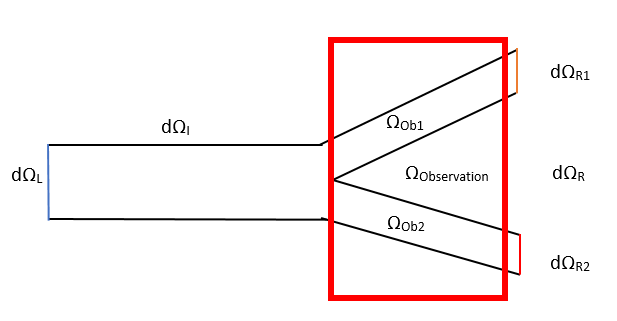
\includegraphics[scale=0.8]{observation.png}
	\caption{Domain of Interest}
	\label{Observation1}
\end{figure}
The first problem of interest is of the form:
\begin{align*}
&\min_{\Sta, w} \quad \frac{1}{2}|| \Sta -\widehat \Sta||^2_{L_2( \Sigma_{Ob})} + \frac{\beta}{2}||w||^2_{L_2(\Sigma)}\\
&\text{subject to:}\\
&\partial_t \rho = \nabla^2 \rho - \nabla \cdot (\rho \mathbf{w}) +\nabla \cdot (\rho \nabla V_{ext}) + \nabla \cdot \int_\Omega \rho(r) \rho(r') \nabla V_2(|r-r'|) dr' + w \quad  \text{in} \quad \Sigma\notag\\
& \rho = \rho_0 \quad \text{at} \quad t=0 \notag\\
& - \mathbf{j} \cdot \nor = \mathbbm{1}_{\partial \Omega_L}( C_{L1}  + C_{L2}\Sta) +\mathbbm{1}_{\partial \Omega_R} ( C_{R1}  + C_{R2}\Sta) +\mathbbm{1}_{\partial \Omega_I} 0 \ \quad \quad\qquad\qquad  \qquad \text{on} \quad \partial \Omega, 
\end{align*}
where $C_{L1}, C_{L2}, C_{R1}$, $C_{R2}$ are constants and $\mathbbm{1}$ is the indicator function of the set of interest. Considering Figure \ref{Observation1}, the stated non-constant flux boundary condition provides the option of describing a non-constant inflow on boundary $\partial \Omega_L$ and a non-constant outflow on $\partial \Omega_R$, while keeping a no flux condition on the rest of the boundary, denoted by $\partial \Omega_I$.
Furthermore, $\mathbf{j}$ satisfies:
\begin{align*}
\mathbf{j}=\nabla \rho - (\rho \mathbf{w}) +(\rho \nabla V_{ext}) +  \int_\Omega \rho(r) \rho(r') \nabla V_2(|r-r'|) dr'.
\end{align*}
Moreover, let $\widehat \Sta$ be defined such that:
\begin{align*}
\widehat \Sta = \mathbbm{1}_{ \Omega_{Ob1}} \tilde \Sta  +\mathbbm{1}_{ \Omega_{Ob2}} 0.
\end{align*}
This describes a desired state where the particle mass accumulates in the observation domain $\Omega_{Ob1}$ and no particles are found in $\Omega_{Ob1}$. Since observations are only taken on $\Omega_{Ob}$, there is no prescribed desired state on $\Omega / \Omega_{Ob}$.\\
The Lagrangian is of the form:
\begin{align*}
\mathcal{L}(\Sta,w,\Adjb,\Adjc ) &=\frac{1}{2} \int_0^T \int_{\Omega_{Ob}} (\Sta - \widehat \Sta)^2 dr dt + \frac{\beta}{2}\int_0^T \int_\Omega w^2 drdt \\
&+ \int_0^T \int_\Omega \bigg( \partial_t \rho - \nabla^2 \rho + \nabla \cdot (\rho \mathbf{w}) -\nabla \cdot (\rho \nabla V_{ext}) \\
&+ \nabla \cdot \int_\Omega \rho(r) \rho(r') \nabla V_2(|r-r'|) -w \bigg) \Adjb dr dt\\
&+ \int_0^T \int_{\partial \Omega} \bigg(  \bigg(-\nabla \rho+ (\rho \mathbf{w}) -(\rho \nabla V_{ext}) -  \int_\Omega \rho(r) \rho(r') \nabla V_2(|r-r'|) dr' \bigg)\cdot \nor\\
&  -\mathbbm{1}_{\partial \Omega_L}( C_{L1}  + C_{L2}\Sta) -\mathbbm{1}_{\partial \Omega_R} ( C_{R1}  + C_{R2}\Sta) -\mathbbm{1}_{\partial \Omega_I} 0 \bigg) \Adjc dr dt.
\end{align*}
The derivative of $\mathcal{L}$ with respect to $\rho$ is, as taken from the extended project, is:
\begin{align*}
&\mathcal{L}_\rho (\rho,{w},\Adjb,\Adjc)h=
\int_\Omega h(T) \Adjb(T) dr\\
&+ \int_0^T \int_\Omega \bigg( \mathbbm{1}_{ \Omega_{Ob}} (\rho- \widehat{\rho})  - \partial_t \Adjb  - \nabla \Adjb \cdot \mathbf{w}  - \nabla^2 \Adjb \notag 
+  \nabla \Adjb \cdot \nabla V_{ext}  \notag \\
&+ \int_\Omega (\nabla  \Adjb(r)+\nabla  \Adjb(r')) \rho(r') \nabla V_2(|r-r'|) dr'+ \int_{\partial \Omega} ( \Adjc(r') - \Adjb(r')) \rho(r')   \frac{\partial V_2(|r-r'|)}{\partial n} dr' \bigg) h dr dt \\
&+  \int_0^T\int_{\partial \Omega}  \bigg(
\bigg(\frac{\partial \Adjb }{\partial n} + \Adjb  \mathbf{w} \cdot \mathbf{n} - \Adjc \mathbf{w} \cdot \mathbf{n}  +  \Adjc \dfrac{\partial V_{ext}}{\partial n} - \Adjb \frac{\partial V_{ext}}{\partial n} + ( \Adjc - \Adjb)  \int_\Omega \rho(r') \frac{\partial V_2(|r-r'|)}{\partial n} dr'\\
& -\mathbbm{1}_{\partial \Omega_L} C_{L2} \Adjc   -\mathbbm{1}_{\partial \Omega_R} C_{R2} \Adjc \bigg)h + \bigg( \Adjc- \Adjb \bigg) \frac{\partial h}{\partial n} \bigg) dr dt =0.
\end{align*}
Then, from appropriate analysis we find that:
\begin{align*}
\Adjc = \Adjb,
\end{align*}
and therefore we get:
\begin{align*}
\mathbbm{1}_{\Omega_{Ob}}(\rho- \widehat{\rho})   - \partial_t  \Adjb  - \nabla \Adjb \cdot \mathbf{w}  - \nabla^2 \Adjb \notag 
+  \nabla \Adjb \cdot \nabla V_{ext}  \notag \\
+ \int_\Omega (\nabla  \Adjb(r)+\nabla  \Adjb(r')) \rho(r') \nabla V_2(|r-r'|) dr' &=0, \quad \text{in} \quad \Sigma, \\
\frac{\partial \Adjb }{\partial n}  -\mathbbm{1}_{\partial \Omega_L} C_{L2} \Adjb   -\mathbbm{1}_{\partial \Omega_R} C_{R2} \Adjb&=0, \quad \text{on} \quad \partial \Omega.
\end{align*}
In particular, this is:
\begin{align*}
\mathbbm{1}_{\Omega_{Ob1}}(\rho- \widehat{\rho}) +\mathbbm{1}_{\Omega_{Ob2}}\rho  - \partial_t  \Adjb  - \nabla \Adjb \cdot \mathbf{w}  - \nabla^2 \Adjb \notag 
+  \nabla \Adjb \cdot \nabla V_{ext}  \notag \\
+ \int_\Omega (\nabla  \Adjb(r)+\nabla  \Adjb(r')) \rho(r') \nabla V_2(|r-r'|) dr' &=0, \quad \text{in} \quad \Sigma, \\
\frac{\partial \Adjb }{\partial n}  -\mathbbm{1}_{\partial \Omega_L} C_{L2} \Adjb   -\mathbbm{1}_{\partial \Omega_R} C_{R2} \Adjb&=0, \quad \text{on} \quad \partial \Omega.
\end{align*}
The gradient equation is:
\begin{align*}
w = \frac{1}{\beta}\Adjb.
\end{align*}
Comparing this to the previous section, it can be observed that the gradient equations have opposite signs. This is due to a different construction of the Lagrangian.





The problem of interest is of the form:
\begin{align*}
&\min_{\Sta, \Con} \quad \frac{1}{2}|| \Sta -\hat \Sta||^2_{L_2(\partial Q_R)} + \frac{\beta}{2}|| \Con||^2_{L_2(Q)}\\
\text{subject to:}\\
&\partial_t \rho = \nabla^2 \rho - \nabla \cdot (\rho \mathbf{w}) +\nabla \cdot (\rho \nabla V_{ext}) + \nabla \cdot \int_\Omega \rho(r) \rho(r') \nabla V_2(|r-r'|) dr' + \Con \quad  \quad\text{in} \quad Q,\notag\\
& \rho = \rho_0 \quad \text{at} \quad t=0 \notag\\
& - \mathbf{j} \cdot \nor = \mathbbm{1}_{\partial \Omega_L}( C_{L1}  + C_{L2}\Sta) +\mathbbm{1}_{\partial \Omega_R} ( C_{R1}  + C_{R2}\Sta) +\mathbbm{1}_{\partial \Omega_I} 0, \quad  \quad\text{on} \quad \partial Q, 
\end{align*}
where $C_{L1}, C_{L2}, C_{R1}$, $C_{R2}$ are constants and $\mathbbm{1}$ is the indicator function of the set (the parts of the boundary) of interest.
Furthermore, $\mathbf{j}$ satisfies:
\begin{align*}
\mathbf{j}=\nabla \rho - (\rho \mathbf{w}) +(\rho \nabla V_{ext}) +  \int_\Omega \rho(r) \rho(r') \nabla V_2(|r-r'|) dr'.
\end{align*}
Moreover, let $\hat \Sta$ be defined such that:
\begin{align*}
\hat \Sta = \mathbbm{1}_{\partial \Omega_{R1}} \tilde \Sta  +\mathbbm{1}_{\partial \Omega_{R2}} 0.
\end{align*}

\subsection*{The Lagrangian}
The Lagrangian is of the form:
\begin{align*}
\mathcal{L}(\Sta,\Con,\Adja,\Adjc ) &= \int_0^T \int_{\partial \Omega_R} \frac{1}{2}(\Sta - \hat \Sta)^2 dr dt + \frac{\beta}{2}\int_0^T \int_\Omega \Con^2 drdt \\
&+ \int_0^T \int_\Omega \bigg( \partial_t \rho - \nabla^2 \rho + \nabla \cdot (\rho \mathbf{w}) -\nabla \cdot (\rho \nabla V_{ext}) + \nabla \cdot \int_\Omega \rho(r) \rho(r') \nabla V_2(|r-r'|) \bigg) \Adja dr dt\\
&+ \int_0^T \int_{\partial \Omega} \bigg(  \bigg(-\nabla \rho+ (\rho \mathbf{w}) -(\rho \nabla V_{ext}) -  \int_\Omega \rho(r) \rho(r') \nabla V_2(|r-r'|) dr' \bigg)\cdot \nor\\
&  -\mathbbm{1}_{\partial \Omega_L}( C_{L1}  + C_{L2}\Sta) -\mathbbm{1}_{\partial \Omega_R} ( C_{R1}  + C_{R2}\Sta) -\mathbbm{1}_{\partial \Omega_I} 0 \bigg) \Adjc dr dt.
\end{align*}

\subsection*{The Adjoint Equation}
The derivative of $\mathcal{L}$ with respect to $\rho$ is, as taken from the extended project:
\begin{align*}
&\mathcal{L}_\rho (\rho,\mathbf{w},p_\Omega,p_{\partial \Omega})h=
\int_\Omega h(T) \Adja(T) dr\\
&+ \int_0^T \int_\Omega \bigg(   - \partial_t \Adja  - \nabla \Adja \cdot \mathbf{w}  - \nabla^2 \Adja \notag 
+  \nabla \Adja \cdot \nabla V_{ext}  \notag \\
&+ \int_\Omega (\nabla  \Adja(r)+\nabla  \Adja(r')) \rho(r') \nabla V_2(|r-r'|) dr'+ \int_{\partial \Omega} ( \Adjc(r') - \Adja(r')) \rho(r')   \frac{\partial V_2(|r-r'|)}{\partial n} dr' \bigg) h dr dt \\
&+  \int_0^T\int_{\partial \Omega}  \bigg(
\bigg(\frac{\partial \Adja }{\partial n} + \Adja  \mathbf{w} \cdot \mathbf{n} - \Adjc \mathbf{w} \cdot \mathbf{n}  +  \Adjc \dfrac{\partial V_{ext}}{\partial n} - \Adja \frac{\partial V_{ext}}{\partial n} + ( \Adjc - \Adja)  \int_\Omega \rho(r') \frac{\partial V_2(|r-r'|)}{\partial n} dr'\\
&\mathbbm{1}_{\partial \Omega_R} (\rho- \hat{\rho}) -\mathbbm{1}_{\partial \Omega_L} C_{L2} \Adjc   -\mathbbm{1}_{\partial \Omega_R} C_{R2} \Adjc \bigg)h + \bigg( \Adjc- \Adja \bigg) \frac{\partial h}{\partial n} \bigg) dr dt =0.
\end{align*}
Then, from appropriate analysis we find that:
\begin{align*}
\Adjc = \Adja,
\end{align*}
and therefore we get:
\begin{align*}
- \partial_t  \Adja  - \nabla \Adja \cdot \mathbf{w}  - \nabla^2 \Adja \notag 
+  \nabla \Adja \cdot \nabla V_{ext}  \notag \\
+ \int_\Omega (\nabla  \Adja(r)+\nabla  \Adja(r')) \rho(r') \nabla V_2(|r-r'|) dr' &=0, \quad \text{in} \quad Q, \\
\frac{\partial \Adja }{\partial n}+ \mathbbm{1}_{\partial \Omega_R} (\rho- \hat{\rho}) -\mathbbm{1}_{\partial \Omega_L} C_{L2} \Adja   -\mathbbm{1}_{\partial \Omega_R} C_{R2} \Adja&=0, \quad \text{on} \quad \partial Q.
\end{align*}
Again, in particular the boundary condition is:
\begin{align*}
\frac{\partial \Adja }{\partial n}+ \mathbbm{1}_{\partial \Omega_{R1}}(\rho- \tilde{\rho} -C_{R2} \Adja) + \mathbbm{1}_{\partial \Omega_{R2}} (\Sta-C_{R2} \Adja) - \mathbbm{1}_{\partial \Omega_L} C_{L2} \Adja   &=0, \quad \text{on} \quad \partial Q.
\end{align*}


\section{Numerical Methods}
In general it is necessary to change the time variable in the adjoint equation, as demonstrated in (++ ++ ), for numerical stability. This is necessary because the forward and adjoint equations contain Laplacians of opposite time. Running the adjoint equation with a negative Laplacian leads to a blow up of the solution at the first time step. The reversal of time, using $\tau = T-t$, remedies this issue, however, this causes a non-local coupling in time between the two PDEs.
The following algorithms provide methods of treating this non-local coupling.


\subsection{Fixed Point Algorithm}\label{sec:Method_SolverFP}
In this section we describe the fixed point algorithm, which is an efficient and stable optimization method for the optimal control problems considered above. 
We denote the discretized versions of the variables $\rho$, $\adj$ and $\vec{w}$ with $P$, $Q$ and $W$, respectively. Each of these matrices is of the form $A = [\boldsymbol{a_0}, \boldsymbol{a_1}, ... ,\boldsymbol{a_n}]$, where the vectors $\boldsymbol{a_k}$ represent the solutions at the discretized times $k \in 0,1,....,n$, where $n$ is the number of time points. In particular, the first column of $P$, denoted by $\boldsymbol{\rho_0}$, corresponds to the initial condition $\rho(r,0)$. If the spatial domain is one-dimensional, $P$, $Q$ and $W$ are of size $N \times (n + 1)$, where $N$ is the number of spatial points. In the two-dimensional case, $P$ and $Q$ are of size $(N_1N_2) \times (n + 1)$, where $N_1$ is the number of spatial points in the direction of $x_1$ and $N_2$ the points along the $x_2$ axis. Generally, $N_1 = N_2$. The discretized control $W$ for linear control problems is also $(N_1N_2) \times (n + 1)$ dimensional, while it is $(2N_1N_2) \times (n + 1)$ dimensional for nonlinear control problems. This is due to the fact that the control is represented by a vector field, when applied nonlinearly.
\\
\\
The optimization algorithm is initialized with a guess for the control, $W^{(0)}$. Then, in each iteration, denoted by $i$, the following steps are computed:
\vspace{0.1cm}
\begin{enumerate}
	\item Starting with a guess for the control $W^{(i)}$ as input variable, the corresponding state $P^{(i)}$ is found by solving the forward equation.
	\item In a next step, the value of the adjoint, $Q^{(i)}$, is established by computing the adjoint equation, using $W^{(i)}$ and $P^{(i)}$ as inputs. Since $P^{(i)}$ contains the solution for all discretized times $k \in 0,1,...,n$, this circumvents issues resulting from the non-local coupling in time, resulting from reversing time in the adjoint equation. As illustrated in the same section, time is reversed in the adjoint equation, so that the result is a matrix $\tilde{Q}^{(i)} =  [\boldsymbol{\adj_n},\boldsymbol{\adj_{n-1}}, ..., \boldsymbol{\adj_1} ]$. The columns of $\tilde{Q}^{(i)}$ are permuted to obtain the solution  $Q^{(i)}$.
	\item The gradient equation is solved, given the solutions $P^{(i)}$ and $Q^{(i)}$. This results in a new value for the control, $W^{(i)}_g$.
	\item  The convergence of the optimization scheme is measured by computing the error between $W^{(i)}$ and $W^{(i)}_{g}$. The error measure, $\mathcal{E}$, is discussed in detail in Section \ref{sec:Method_Validation}. 
	\begin{itemize}
		\item  If this error is lower than a set tolerance, the optimality system is self-consistent. This implies that the solution triplet ($\bar{P},\bar{W},\bar{Q}$) solves the (discretized) optimality system, and is therefore an optimal solution to the PDE-constrained optimization problem of interest.
		\item If the error is above the optimality tolerance, step 5 is executed.
	\end{itemize}
	\item Finally, the update $W^{(i+1)}$ is a linear combination of the current guess $W^{(i)}$, and the value obtained in step 3, $W^{(i)}_{g}$, employing a mixing rate $\lambda \in [0,1]$:
	\begin{align*}
	W^{(i+1)} = (1-\lambda)W^{(i)} + \lambda W^{(i)}_{g}.
	\end{align*}
	The guess for the control is updated from $W^{(i)} $ to $W^{(i+1)} $ and steps 1-5 are repeated until the method converges. 
\end{enumerate}
\vspace{0.3cm}
The update scheme in step 5, with mixing rate $\lambda$, is known to stabilise fixed point methods, ++Ben to add references++. Typical values of $\lambda$, which provide stable convergence, lie between $0.1$ and $0.001$. Throughout this paper, $\lambda =0.01$, unless stated otherwise. This mixing scheme is similar to the updating scheme presented in~\cite{Burger1}. 
Note that, while the solutions $P^{(i)}$ and $Q^{(i)}$ change in each iteration, the initial condition $\boldsymbol{\rho_0}$ and final time condition $\boldsymbol{\adj_n}$ remain unchanged throughout the process. Therefore, the only variable inducing a change in the solution is $W^{(i)}$.
\subsection{Picard Multiple Shooting}

The multiple shooting algorithm, introduced in the first year report, has been extended by employing a Picard mixing scheme as optimization method to replace the {\scshape MATLAB} inbuilt solver \texttt{fsolve}. In the following, this is briefly outlined.
The idea of the updating scheme is similar to the one presented for the fixed point algorithm. However, while the multiple shooting algorithm updates through the variables $\rho$ and $q$, the fixed point algorithm updates through the control variable.
The multiple shooting method consists of discretizing the time interval and solving the optimality system on each interval individually. This is done because of the non-local time coupling of the forward and adjoint equations. It requires the input of an initial guess at each time for each of the variables. The aim of the optimization solver is then to minimize the distance between the initial guesses and numerical solutions of the variables at each of the time points. \\
The Picard mixing scheme is a fixed point type algorithm. At each iteration $i$ it takes a set of guesses at the discretized time points, denoted by $Y_i$. The matrix $Y = [P,Q]$ contains the discretized values for the variables $\rho$ and $q$, denoted by $P$ and $Q$, analogously to the previous section.  
The system of PDEs on the discretized intervals is computed and a new set of variable values at the time points is created, denoted by $Y_{out}$. Then, the mixing scheme provides a new guess for the iteration $i+1$ by:
\begin{align*}
Y_{i+1} = (1 - \lambda)Y_i + \lambda Y_{out},
\end{align*}
where $\lambda$ is the mixing rate. It typically takes values between $0.1$ and $0.01$, depending on the complexity of the system to solve. Choosing a relatively small value of $\lambda$ stabilizes the algorithm (+ ref this?+). 
The algorithm terminates when the system of PDEs is solved self-consistently, i.e. when the distance between $Y_i$ and $Y_{out}$ is small, as measured in a chosen norm. The most frequently applied norm is discussed in Section \ref{sec:ErrorMeasure}.
This algorithm is working very well for examples involving the overdamped equations. However, the fixed point algorithm provides an even simpler method, which does not require the solution of the optimality system on small time intervals and is therefore even quicker. Since we will apply the numerical optimization method to increasingly difficult optimal control problems in the future, the multiple shooting algorithm may provide more numerical stability for numerically harder problems and is therefore a relevant tool to consider in the future. Changing the optimization solver in the implementation is straightforward and requires only changing a flag in the input file.
\\
A challenge with this solver is that it needs to be provided with good initial guesses for the variables $\rho$ and $\adj$ at the discretized time points. The guess for $\rho$ can be obtained by solving the associated forward problem and using the result as a first guess. However, a good guess for $\adj$ is trickier to achieve. One way of doing so is by using the gradient equation, which relates $\rho$, $\adj$ and $w$, the control. Since the input for the forward control is known, one can use this information, together with the initial guess for $\rho$ to construct an initial guess for $\adj$. 
One challenge however arises when considering the flow control problem involving the overdamped equations. The gradient equation is $\mathbf{w} = - \frac{1}{\beta} \rho\nabla \adj$. In order to derive the value of $\adj$ from this equation, we need to divide by $\rho$, making use of the assumption that $\rho$ is strictly positive, and integrate over the whole space. The issue here is that integration introduces an indeterminable constant. Furthermore, if Dirichlet boundary conditions are applied, the strict positivity of $\rho$ is in question.\\
Alternatively, one step of the fixed point method could be performed initially, to obtain an initial guess for $\adj$. 


\subsection{{\scshape MATLAB}'s Inbuilt Optimization Solver \texttt{fsolve}}
Another option of solving the optimality system is using the inbuilt {\scshape MATLAB} solver \texttt{fsolve} in combination with the multiple shooting method briefly described in the previous section. The optimization solver tries to minimize the error in the variables $\rho$ and $\adj$ at the discretized time points. 
\\
In general, for the set of non-linear functions, $F(x)$, that are supposed to be solved, \texttt{fsolve} tries to find an input vector $x$, such that we minimize sum of squares $\sum_i f_i(x)^2$, where $f_i$ are the components of $F$. 
While \texttt{fsolve} has three different algorithm options, the default is the trust region dogleg algorithm, a variant of Powell's dogleg algorithm (++ ref++).   
The general idea of trust-region algorithms is to consider a so-called trust-region $N$, in which the function $F$ is approximated by a simpler function. Then, a search direction $s$ is defined and it is decided whether $F(x+s) < F(x)$. If that is the case, the position $x$ is updated to the position $x+s$. Otherwise, we remain at the position $x$ and the trust region $N$ is made smaller.
The main questions are (i) how to approximate the function in the trust region, and (ii) how to determine the search direction $s$ reliably.\\
In the case of the dogleg algorithm, the choice for (i) is to minimize:
\begin{align}
\label{eqn:trustregionsubprob1}
\min_s m(s) &= \frac{1}{2}|| F(x_k) + J(x_k)s||_2^2 \\
&= \frac{1}{2}F(x_k)^T F(x_k) + s^T J(x_k)^T F(x_k) + \frac{1}{2}s^T J(x_k)^TJ(x_k)s, \notag
\end{align}
where $J$ is the Jacobian.
In order to minimize $m$, we choose, answering (ii), the appropriate search direction $s$. In the dogleg method this is done by combining a Gauss-Newton step $s_{GN}$ with a Cauchy step $s_C$.
If $J(x_k)$ is singular, $s = s_C$. Otherwise, $s$ is chosen as a linear combination of these two steps as:
\begin{align*}
s = s_C + \lambda(s_{GN} - s_C),
\end{align*}
where $\lambda \in [0,1]$ is the largest value such that $||s|| \leq \Delta$. The positive scalar $\Delta$ is the trust region dimension, and adjusted at each iteration. The algorithm converges when $F(x)$ and $F(x+s)$ are close. 
While this method is more stable than a Newton method, and the initial guess for the algorithm does not have to be as good, and it is cheaper to compute, it is also prone to converging to local minima, since we do not consider the whole domain.
(++ ref with matlab pages ++)
\section{Investigating Functionality of the Optimization Algorithms}

\subsection{Error Measure}\label{sec:ErrorMeasure}
While other norms such as an $L_1$ norm or a pointwise error measure have been considered, the main measure employed in this work is the following.

All errors in Sections +++ are calculated between a variable of interest, $y$, and $y_R$, the reference value that $y$ is compared to. When measuring convergence of the fixed point scheme, described in Section \ref{sec:Method_SolverFP}, $y = W^{(i)}_g$ and $y_R = W^{(i)}_i$. Alternatively, when investigating a known test problem, $y$ is a numerical solution and $y_R$ is an exact solution. The error measure $\mathcal{E}$ is composed of an $L^2$ error in space and an $L^\infty$ error in time. The relative $L^2$ error in the spatial direction is:
\begin{align*}
\mathcal{E}_{Rel}(t) = \frac{|| y(x,t) - y_{R}(x,t)||_{L^2(\Omega)} }{||y_R(x,t) ||_{L^2(\Omega)}+ 10^{-10}},
\end{align*}
where the small additional term on the denominator prevents division by zero.
Furthermore, the absolute $L^2$ error is:
\begin{align*}
\mathcal{E}_{Abs}(t) = || y(x,t) - y_R(x,t)||_{L^2(\Omega)}.
\end{align*}
Then, an $L^\infty$ error in time is taken of the minimum of $\mathcal{E}_{Rel}$ and $\mathcal{E}_{Abs}$, to obtain the error of interest:
\begin{align*}
\mathcal{E} = \max_{t \in [0,T]}\left[\min\left(\mathcal{E}_{Rel}(t), \mathcal{E}_{Abs}(t)\right)\right].
\end{align*}
The minimum between absolute and relative spatial error is taken to avoid choosing an erogenously large relative error, caused by division of one small term by another.




\subsection{Validation against \texttt{fsolve}}
As a benchmark, we compared the fixed point scheme to Matlab's inbuilt \texttt{fsolve} function. It uses the trust-region-dogleg algorithm, see~\cite{Powell1}, to solve the optimality system of interest. While it is very robust, it is also much slower than the fixed point method, which works reliably for the types of problems considered. 

Example 1 in Section \ref{sec:Examples1d} is considered to compare the computational time taken of the fixed point algorithm and the inbuilt Matlab function \texttt{fsolve}. Note that the comparison is slightly impacted by the fact that convergence is measured differently in these two numerical methods. However, a general comparison can be made regarding the efficiency of the two approaches.
We choose $n=20$, $N=30$, the ODE solver tolerance is set to be $10^{-8}$, the optimality tolerance is $10^{-4}$ and $\beta = 10^{-3}$. 
As can be seen in Table \ref{TabA3:Prob11}, the running time of the fixed point algorithm is considerably faster than for \texttt{fsolve}, while the resulting values of the cost functional remain the same. This can be confirmed by comparing the number of function evaluations for each method, which is an important measure when dealing with large systems, such as the two-dimensional problems discussed in this paper, since each iteration is costly for large problems. The differences in $\rho$ and $\adj$ are broadly in line with the optimality tolerance, however the control differs more, because $\mathbf{w}$ is updated using the optimal values of $\rho$ and $\adj$. 
%
\begin{table}
\begin{tabular}{ | c | c || c | c | c ||}
\hline
\multicolumn{2}{|c||}{} & Fixed Point & \texttt{fsolve} & Difference   \\
\hline
\hline
 & $\mathcal{J}_{uc}$ & $\numprint{0.0438}$ & $\numprint{0.0438}$ &   \\
 & $\mathcal{J}_{c}$ & $\numprint{0.0011}$ & $\numprint{0.0011}$ &   \\
 & \texttt{Iter} (\texttt{funcEval}) & $\numprint{670}$ ($\numprint{670}$)  & $\numprint{38}$ ($\numprint{31959}$)  &   \\
$\kappa =-1$ & Time taken (s) & $\numprint{2.4939e+2}$ & $\numprint{9.1546e+3}$ &   \\
 & $\mathcal{E}_{\rho_{Diff}}$ & & &$\numprint{1.1348e-3}$  \\
 & $\mathcal{E}_{\adj_{Diff}}$ & & &$\numprint{7.2742e-5}$  \\
 & $\mathcal{E}_{\mathbf{w}_{Diff}}$ & & & $\numprint{7.6725e-2}$  \\
\hline
 & $\mathcal{J}_{uc}$ & $\numprint{0.0434}$ & $\numprint{0.0434}$ &   \\
 & $\mathcal{J}_{c}$ & $\numprint{0.0020}$ & $\numprint{0.0020}$ &   \\
 & \texttt{Iter} (\texttt{funcEval}) & $\numprint{654}$ ($\numprint{654}$)  & $\numprint{38}$ ($\numprint{34239}$)  &   \\
$\kappa =1$ & Time taken (s) & $\numprint{3.3794e+2}$ & $\numprint{1.0167e+4}$ &   \\
 & $\mathcal{E}_{\rho_{Diff}}$ & & &$\numprint{3.0610e-4}$  \\
 & $\mathcal{E}_{\adj_{Diff}}$ & & &$\numprint{4.8701e-5}$  \\
 & $\mathcal{E}_{\mathbf{w}_{Diff}}$ & & & $\numprint{8.9056e-3}$  \\
\hline
\end{tabular}
\caption{Comparison of the outputs of the fixed point method, with those obtained using \texttt{fsolve}.}
\label{TabA3:Prob1}
\end{table} \label{TabA3:Prob11}


\subsection{Perturbing $w$}

As detailed in Section \ref{sec:Method_SolverFP}, it is necessary to provide an initial guess for the control $\mathbf{w}$ to start the optimization routine. Therefore, one way of validating the numerical method is to perturb the exact solution for $\mathbf{w}$, taken from a test problem with analytic solution, and use this as an initial guess in the optimization solver. In the first iteration, the solutions for $\rho$ and $\adj$ differ from the exact solution. The optimization method then converges to the exact, optimal solution. We consider an exact solution for the overdamped flow control problem \eqref{eqn:ADFlowOCP}, with no-flux boundary conditions, and no particle interaction term. This specific exact solution can be found in our paper's supplementary material (Section A), called Test Problem 2. 
The following two perturbation functions are considered. The first perturbation is in time only and is defined as:
\begin{align*}
g(t) &= \frac{1}{2} f(t-t_0, a) \times f(t-t_0, -a)\\
&= \frac{1}{2} \frac{e^{-a/(t-t_0)}}{e^{-a/(t-t_0)} + e^{-a/(1-t -t_0)}} \times \frac{e^{a/(t-t_0)}}{e^{a/(t-t_0)} + e^{a/(1-t - t_0)}},
\end{align*}
and normalised by:
\begin{align*}
\tilde g(t) = \frac{g(t)}{\max{|{g(t)}|}}.
\end{align*}
A similar perturbation can be done in space, taking into account the difference in length of spatial and time domains:
\begin{align*}
h(x) &= \frac{1}{2} f(x-x_0, 2a) \times f(x-x_0, -2a)\\
&= \frac{1}{2} \frac{e^{-2a/(x-x_0)}}{e^{-2a/(x-x_0)} + e^{-2a/(1-x-x_0)}} \times \frac{e^{2a/(x-x_0)}}{e^{2a/(x-x_0)} + e^{2a/(1-x-x_0)}}.
\end{align*}
Again, this is normalised:
\begin{align*}
\tilde h(x) = \frac{h(x)}{\max{|{h(x)}|}}.
\end{align*}
These perturbation functions are chosen such that the perturbation is smooth and respects the initial condition for $\rho$, as well as the final time condition for $\adj$, by not changing the first or final time point. If this is not respected, the algorithm converges up to a point and then diverges, since the boundary conditions in time cannot be matched.
The considered perturbations are applied to the exact solution of the control, $\mathbf{w}_{ex}$, as follows:
\begin{align*}
\mathbf{w}_{pert1} &= \mathbf{w}_{ex}(1+ \epsilon \tilde g(t))\\
\mathbf{w}_{pert2} &= \mathbf{w}_{ex}(1+ \epsilon \tilde g(t) \tilde h(x)),
\end{align*}
where $a = 0.7$, $x_0 = t_0 = -0.01$ and the perturbation strength is either $\epsilon = 0.1$ or $\epsilon = 0.5$.
The chosen number of points is $N =30$ and $n=20$, the ODE tolerances are $10^{-8}$ and the optimality tolerance is $10^{-4}$. The mixing rate for the optimization solver is $\lambda = 0.01$.
The results presented in Table \ref{TabA2:Prob11} show the initial error in $\mathbf{w}$, $\mathcal{E}_{\mathbf{w}_{uc}}$, and the final errors in $\mathbf{w}$, $\rho$ and $\adj$, measured in the norm presented in Section \ref{sec:ErrorMeasure}, with respect to the exact solution. The initial error $\mathcal{E}_{\mathbf{w}_{uc}}$ is proportional to the perturbation strength $\epsilon$. The final errors for $\mathbf{w}$ and $\rho$ and $\adj$ are mostly within the specified optimality tolerance regardless of the perturbation strength and location. 

\begin{table}
\begin{tabular}{ | c | c || c | c | c | c ||}
\hline
  \multicolumn{2}{|c||}{} & $\beta = 10^{-3}$ & $\beta = 10^{-1}$ & $\beta = 10^{1}$ & $\beta = 10^{3}$  \\
\hline
\hline
\multirow{4}{*}{$0.1 \tilde g(t)$} & $\mathcal{E}_{\mathbf{w}_{uc}}$ & $\numprint{1.0000e-1}$ & $\numprint{1.0000e-1}$ & $\numprint{1.0000e-1}$ & $\numprint{1.0000e-1}$ \\
 & $\mathcal{E}_{\mathbf{w}_c}$ & $\numprint{5.3770e-5}$ & $\numprint{5.2340e-5}$ & $\numprint{5.2201e-5}$ & $\numprint{5.2203e-5}$ \\
 & $\mathcal{E}_{\rho}$ & $\numprint{1.1396e-5}$ & $\numprint{7.8597e-5}$ & $\numprint{7.8595e-5}$ & $\numprint{7.8597e-5}$ \\
 & $\mathcal{E}_{\adj}$ & $\numprint{2.7854e-5}$ & $\numprint{2.7836e-4}$ & $\numprint{5.7043e-4}$ & $\numprint{5.7045e-4}$ \\
\hline
\multirow{4}{*}{$0.5 \tilde g(t)$} & $\mathcal{E}_{\mathbf{w}_{uc}}$ & $\numprint{5.0000e-1}$ & $\numprint{5.0000e-1}$ & $\numprint{5.0000e-1}$ & $\numprint{5.0000e-1}$ \\
 & $\mathcal{E}_{\mathbf{w}_c}$ & $\numprint{2.1970e-4}$ & $\numprint{2.1747e-4}$ & $\numprint{2.1735e-4}$ & $\numprint{2.1735e-4}$ \\
 & $\mathcal{E}_{\rho}$ & $\numprint{2.4256e-5}$ & $\numprint{2.2878e-4}$ & $\numprint{2.2878e-4}$ & $\numprint{2.2879e-4}$ \\
 & $\mathcal{E}_{\adj}$ & $\numprint{3.3247e-5}$ & $\numprint{3.3227e-4}$ & $\numprint{6.8088e-4}$ & $\numprint{6.8090e-4}$ \\
\hline
\multirow{4}{*}{$0.1 \tilde h(x)$} & $\mathcal{E}_{\mathbf{w}_{uc}}$ & $\numprint{8.5568e-2}$ & $\numprint{8.5568e-2}$ & $\numprint{8.5568e-2}$ & $\numprint{8.5568e-2}$ \\
 & $\mathcal{E}_{\mathbf{w}_c}$ & $\numprint{5.3700e-5}$ & $\numprint{5.2250e-5}$ & $\numprint{5.2100e-5}$ & $\numprint{5.2103e-5}$ \\
 & $\mathcal{E}_{\rho}$ & $\numprint{1.1704e-5}$ & $\numprint{7.7973e-5}$ & $\numprint{7.7969e-5}$ & $\numprint{7.7968e-5}$ \\
 & $\mathcal{E}_{\adj}$ & $\numprint{2.6426e-5}$ & $\numprint{2.6387e-4}$ & $\numprint{5.6982e-4}$ & $\numprint{5.6984e-4}$ \\
\hline
\multirow{4}{*}{$0.5 \tilde h(x)$} & $\mathcal{E}_{\mathbf{w}_{uc}}$ & $\numprint{4.2784e-1}$ & $\numprint{4.2784e-1}$ & $\numprint{4.2784e-1}$ & $\numprint{4.2784e-1}$ \\
 & $\mathcal{E}_{\mathbf{w}_c}$ & $\numprint{2.1203e-4}$ & $\numprint{2.0982e-4}$ & $\numprint{2.0967e-4}$ & $\numprint{2.0968e-4}$ \\
 & $\mathcal{E}_{\rho}$ & $\numprint{2.2565e-5}$ & $\numprint{2.1275e-4}$ & $\numprint{2.1274e-4}$ & $\numprint{2.1275e-4}$ \\
 & $\mathcal{E}_{\adj}$ & $\numprint{3.0225e-5}$ & $\numprint{3.0219e-4}$ & $\numprint{6.1920e-4}$ & $\numprint{6.1923e-4}$ \\
\hline
\end{tabular}
\caption{Error measures for $\mathbf{w}_{uc}$, $\mathbf{w}_{c}$, $\rho$, and $\adj$, for four perturbation strategies for $\mathbf{w}$, and a range of $\beta$.}
\label{TabA2:Prob1}
\end{table} \label{TabA2:Prob11}

\subsection{Additional Observations}
In the following, a few further observations are stated, that were made when applying the optimization solver to problems involving the overdamped equations. Demonstrations of these points are omitted due to time constraints and will be provided in future work.
During the investigation of different perturbed exact problems and other test problems, it could be observed that the weakness of the optimization method lies in solving advection dominant problems. 
This became apparent when considering different analytic exact solutions to the overdamped flow control problem \eqref{eqn:ADFlowOCP}. Depending on the magnitude of the control in each problem, the algorithm could either converge or not. Scaling the size of the control down, it was possible to achieve convergence for problems that were previously too difficult for the optimization solver. Another way of achieving convergence is to introduce a diffusion coefficient into the problem. A large advection term can then be offset with a large diffusion coefficient and the optimization solver is able to converge.
The issue of advection dominance is especially prevalent when applying no-flux boundary conditions. This is because in order to match the boundary conditions in an advection dominated problem, the gradients of the particle distributions become steep at the boundary. Since steep gradients are difficult to treat numerically, this is an exacerbation of the problem at hand.
It is important to point out that this issue is encountered with any optimization and forward solvers and is not unique to our choice of methods. 
\\
\\
During the work on the overdamped equations it was found that one limiting factor in the convergence of the method is interpolation errors. The error made during interpolation is of order $10^{-8} - 10^{-9}$. Therefore, the ODE solver cannot be more accurate than that and consequently the optimization error has to be adapted to this finding as well.
Furthermore, the optimization tolerance has to be chosen in such a way that it takes into account the accumulation of error during the ODE solves and with each iteration of the optimization algorithm. This results in the optimization tolerance to be at least three orders larger than the ODE solver tolerance, which is bounded by the interpolation error. We found that in general choosing the ODE solver tolerance to be $10^{-8}$ and the optimization tolerance to be $10^{-4}$ we get reliable convergence for most test problems.
\\
Another thing to take into consideration is that the problem becomes numerically harder with decreasing value of $\beta$. In general, small $\beta$ may need more points to be solved to the same accuracy as larger values of $\beta$, or may not reach the same accuracy at all. (++ See examples ++).


\section{Examples}

+++  copied from paper draft. fix +++
In order to solve the optimal control problems \eqref{AdvDiff} and \eqref{AdvDiff_Linear}, some inputs must be provided. The desired state $\widehat \rho$, the PDE source term $f$, and the external potential $V_{ext}$ must be given. Furthermore, an initial condition for $\rho$, the final time condition for $\adj$ and an initial guess for the control $\vec{w}$ have to be be specified. 
The interaction kernel (++ terminology? ++) is of the form:
\begin{align*}
\vec{K} = \nabla V_2, \qquad V_2 = e^{-x^2}.
\end{align*}
Three interaction strengths are considered in this section. Firstly, each problem is solved without an interaction term present ($\gamma = 0$). Then, the considered problem is solved with an order one attractive interaction term ($\gamma = -1$) and an order one repulsive interaction term ($\gamma = 1$), respectively. Initially, the control $\vec{w}$ is set to zero. It is then investigated how the control changes from this baseline, influenced by the different interaction strengths. 
Initially the forward PDE is solved, using the initial configuration $\vec{w}=0$ and the cost functional $J$ is evaluated at this initial state and denoted by $J_I$. Note that no optimization methods are used to derive this value. We then expect that applying the optimization method lowers the value of the cost functional, which we aim to minimize. 
In particular, the value of the optimal cost functional, denoted by $J_O$, is lower the more control is allowed to enter the system though the optimization process. 
This depends on the value of the regularization parameter $\beta$ and it is expected that the control will increase with decreasing $\beta$, since the cost functionals in problems \eqref{AdvDiff} and \eqref{AdvDiff_Linear} allow for a larger control with smaller $\beta$. 

In the following examples, the domain considered is $\Omega \times [0,T] = [-1,1] \times [0,1]$. The number of spatial points is $N=30$ in one-dimensional examples, $N_1 = N_2 = 30$ in two-dimensional examples, and the number of time points is $n=20$, unless stated otherwise. The tolerances in the ODE solver are set to $10^{-8}$ and the tolerance for the convergence of the optimization algorithm is $10^{-4}$. The mixing parameter $\lambda$ is $0.01$, unless stated otherwise.
\subsection{Nonlinear control problems with an additional nonlocal integral term in 1D} \label{sec:Examples1d}
Examples of solving Problem \eqref{AdvDiff}, with 'no-flux type'/Neumann boundary conditions \eqref{NoFlux} and Dirichlet boundary conditions \eqref{Dirichlet} are given in this section. 
 
\subsubsection{Neumann boundary conditions, Example 1}	 
The chosen inputs for this example are:
\begin{align*}
&\widehat \rho = \frac{1}{2}(1-t) + t\bigg(\frac{1}{2}\sin(\pi (y - 2)/2) + \frac{1}{2}\bigg),\\
&\rho_{0} = \frac{1}{2}, \ \
\adj_{T} = 0, \ \
\vec{w} = \vec{0}, \ \ 
f =0,\ \
V_{ext} =0.
\end{align*}	
The value of the cost functional for the initial configuration ($J_{I}$), where $\vec{w} =0$, is compared with the optimized case ($J_{O}$) for different values of $\beta$ and for each of the interaction strengths in Table \ref{TabS5:Prob1}. It can be observed that in all cases $J_{O}$ is lower or equal value to $J_{I}$. The lowest values of $J_{O}$ will be observed for the smallest $\beta$ value considered. At large values of $\beta$, applying control is heavily penalised and the optimal control approaches zero, which coincides with the uncontrolled case. Furthermore, this is reflected in the number of iterations, which is small when $\beta$ is large, and vice versa. This is explained by the fact that if applying control is penalized heavily, then $\vec{w} = 0$ is a better initial guess, and less iterations are needed to find the optimal solution, than when $\beta$ is small and more control is allowed.

 The desired state $\widehat \rho$, and the uncontrolled state $\rho$ for $\gamma =1$ and $\gamma = -1$ are shown in Figure \ref{Ex12DN1}. These two variables are independent of $\beta$. However, $\rho$ changes considerably with the choice of interaction strength $\gamma$, accumulating mass in the centre of the domain for attractive interactions and at the boundary for repulsive interactions. The optimal states $\rho$ for $\gamma = 1,0,-1$ and corresponding optimal controls, with $\beta = 10^{-3}$, are shown in Figure \ref{Ex12DN2}. 
It can be observed that in the case of $\beta = 10^{-3}$, the optimal state $\rho$ is very similar to $\hat \rho$, regardless of the choice of interaction. However, the corresponding control plot reveals that the control has to be applied differently in each case to account for the interaction effects. In general, the control is largely applied on the right half of the spatial domain, to carry mass to the left, where the desired state dictates it to be, as can be seen when $\gamma = 0$. However, when the particle interaction is repulsive, the control is moving some of the particle mass away from the boundary at $x=-1$ to correct for the repulsive particles accumulating there without control present, as illustrated in Figure \ref{Ex12DN1}. In the attractive case, the control corrects by carrying some mass to the boundary at $x=1$, since the uncontrolled particle density is clustered in the middle of the domain in this case, compare to Figure \ref{Ex12DN1}.
\begin{figure}[h]
	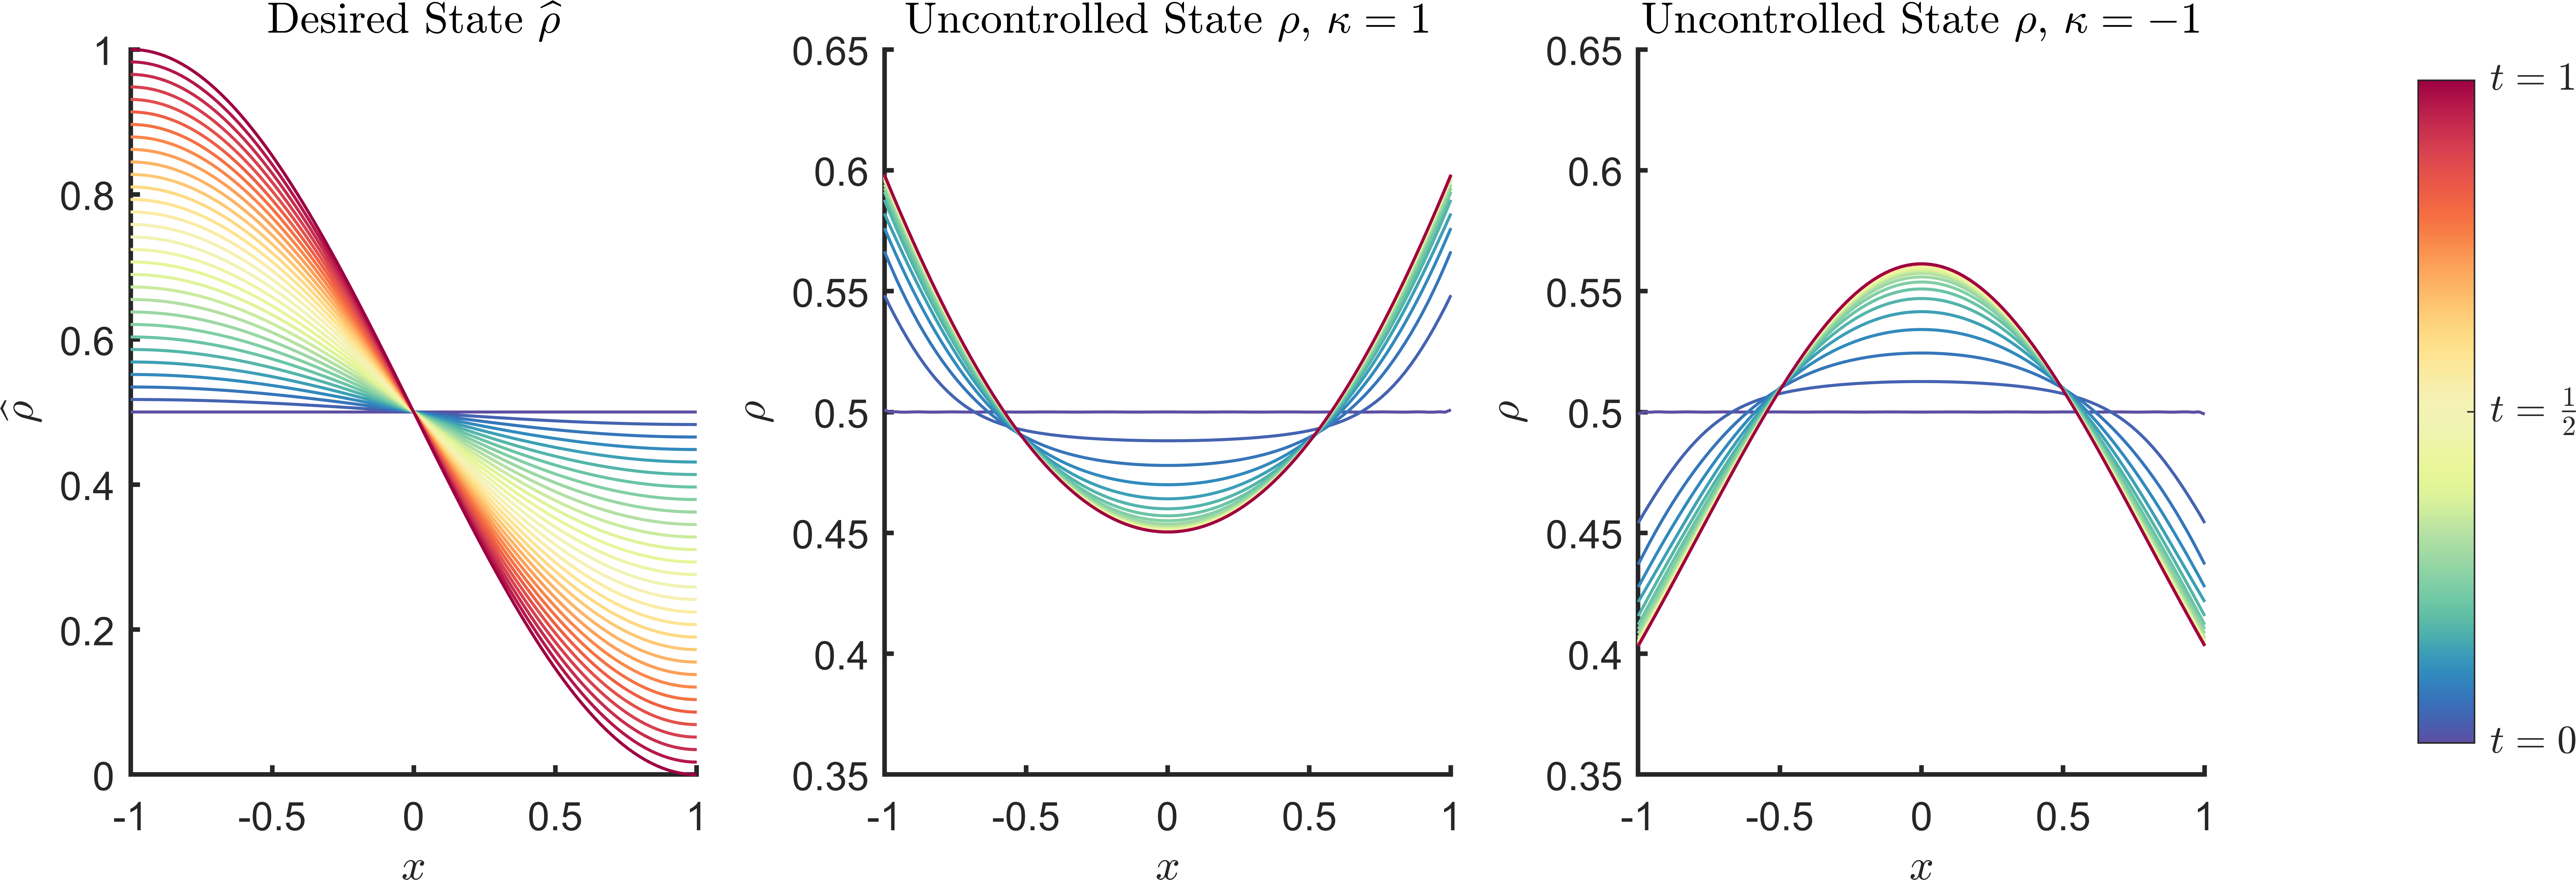
\includegraphics[scale=0.05]{Figure1.png}
	\caption{Example 1, desired state $\widehat \rho$ and uncontrolled state $\rho$ at $\gamma =1$ and $\gamma =-1$}
	\label{Ex12DN1}
\end{figure}
\begin{figure}[h]
	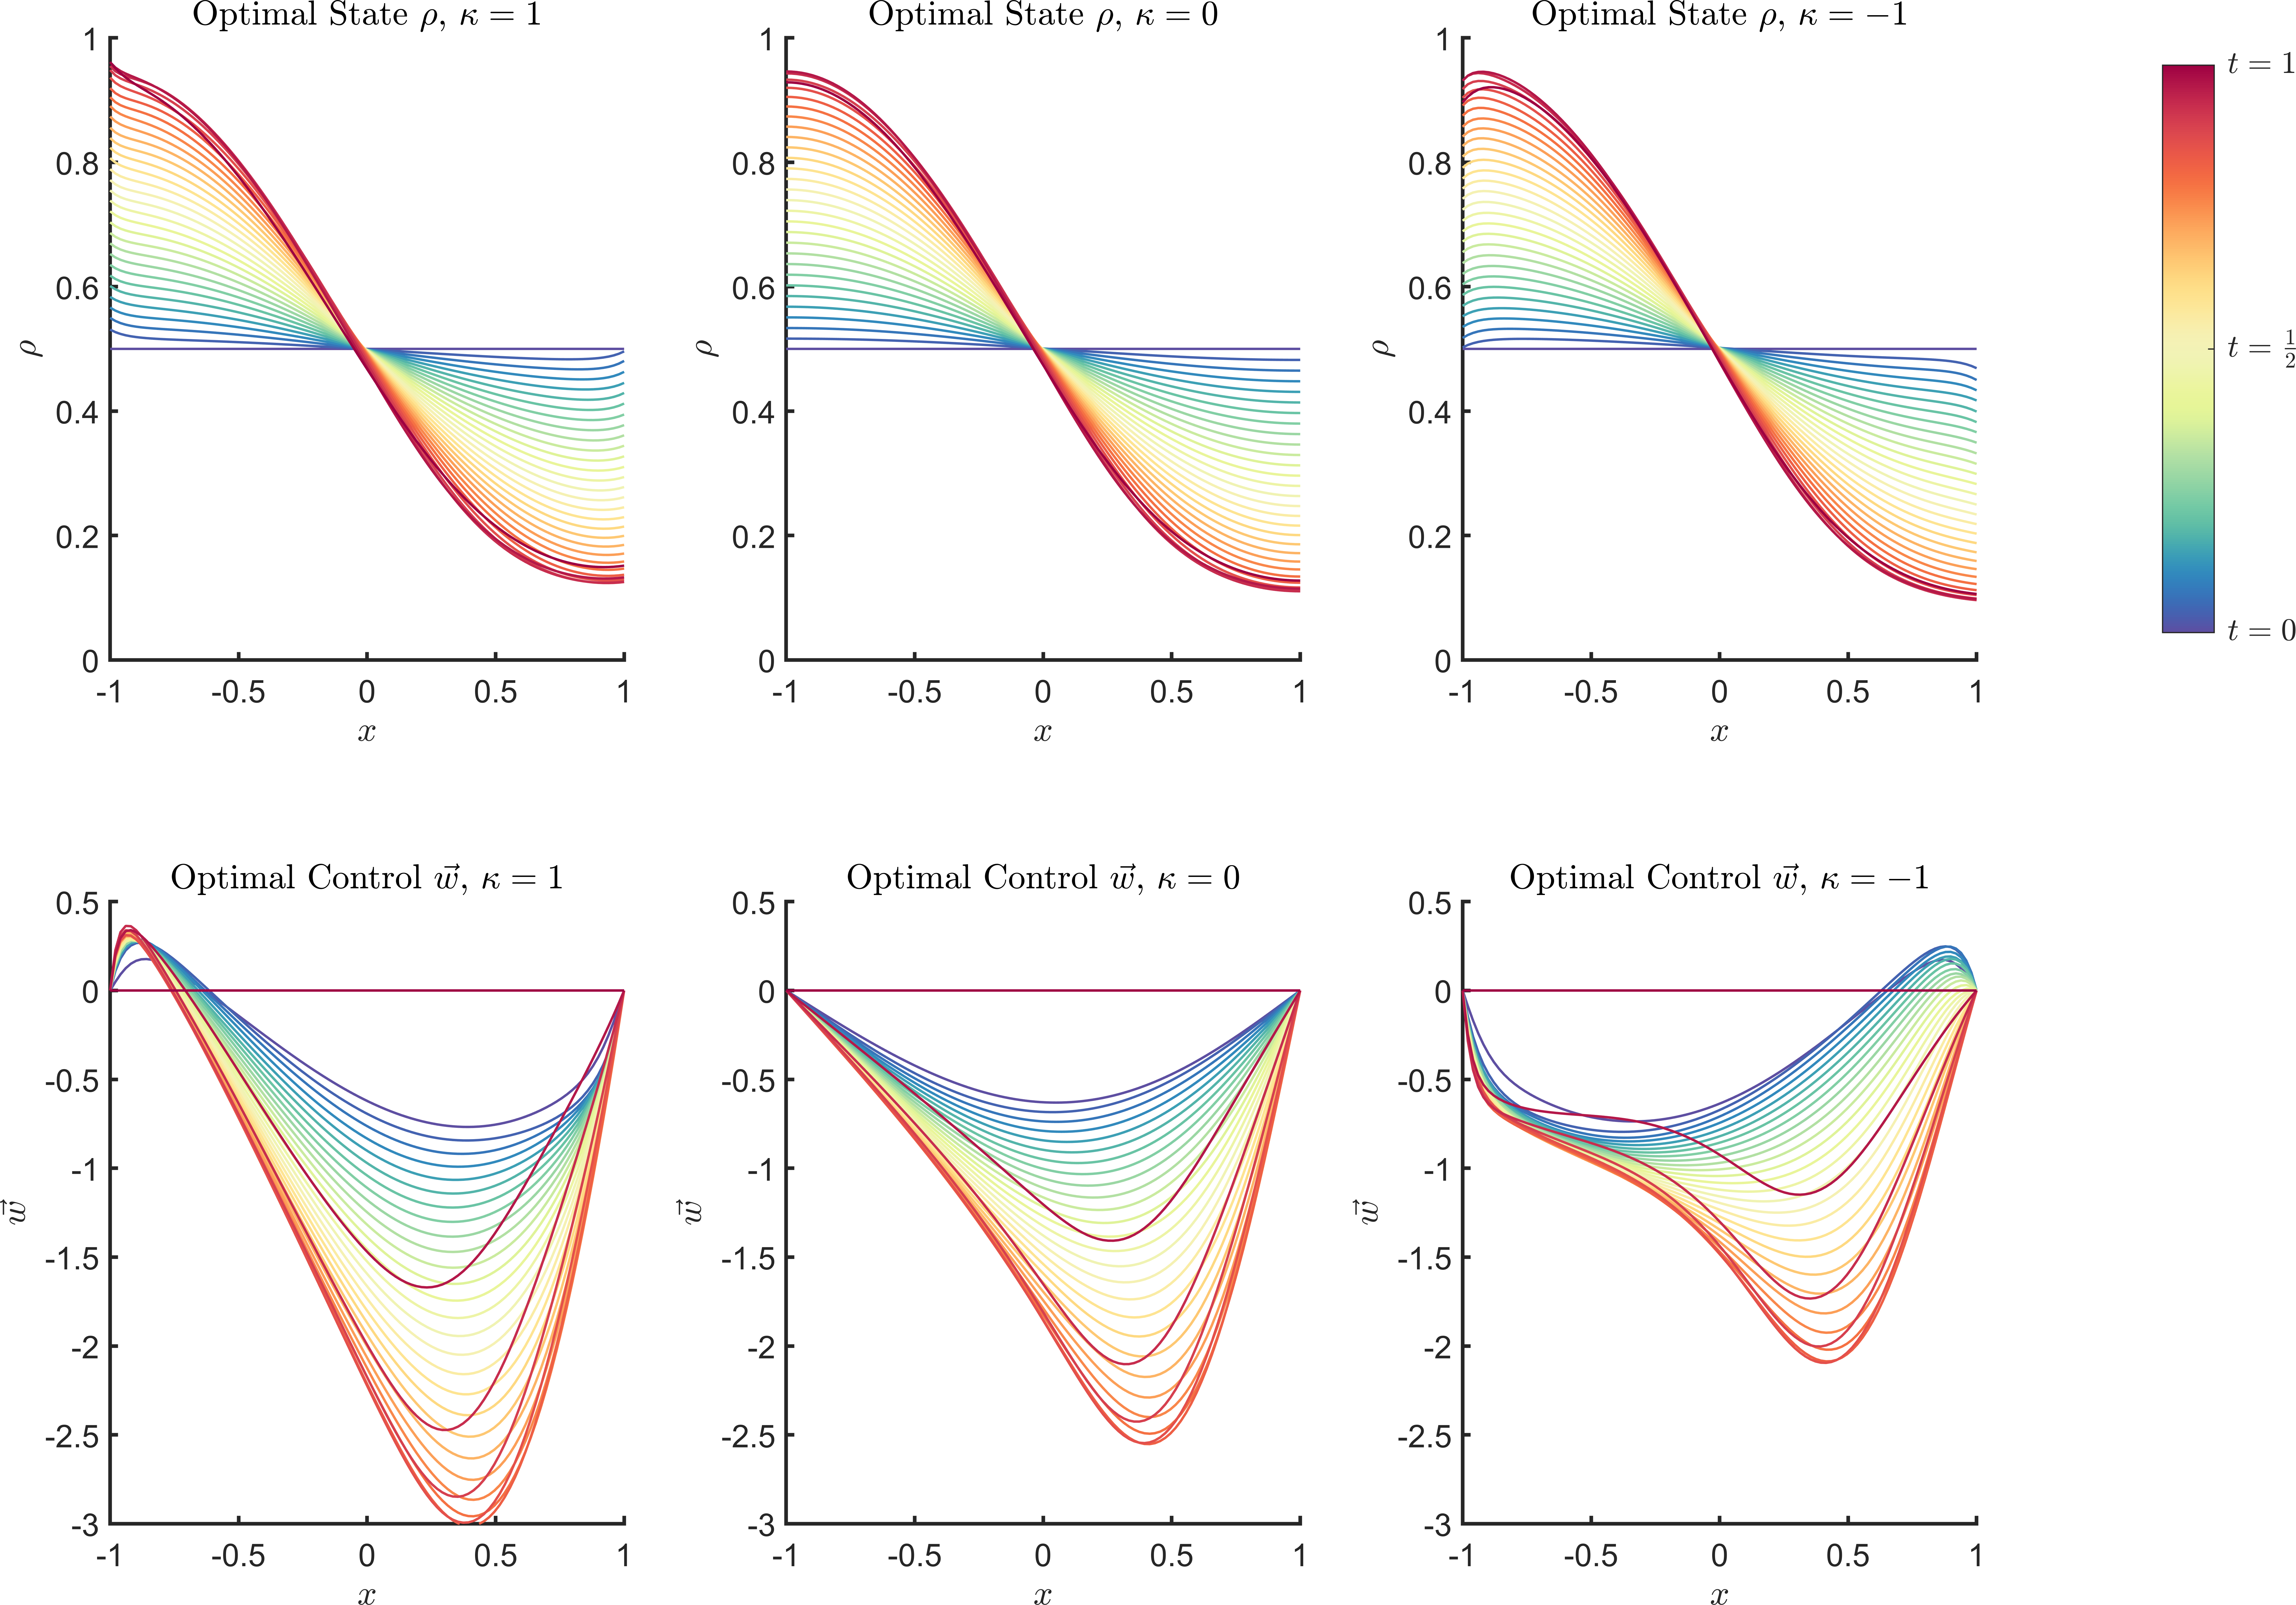
\includegraphics[scale=0.05]{Figure2.png}
	\caption{Example 1, optimal state $\rho$ and the corresponding optimal control $\vec{w}$ for $\gamma = 1,0,-1$, $\beta = 10^{-3}$.}
	\label{Ex12DN2}
\end{figure}

\begin{table}
\begin{tabular}{ | c | c || c | c | c | c ||}
\hline
\multicolumn{2}{|c||}{}& $\beta = 10^{-3}$ & $\beta = 10^{-1}$ & $\beta = 10^{1}$ & $\beta = 10^{3}$  \\
\hline
\hline
 & $\mathcal{J}_{uc}$ & $\numprint{0.0438}$ & $\numprint{0.0438}$ & $\numprint{0.0438}$ & $\numprint{0.0438}$ \\
$\kappa= \numprint{-1}$  & $\mathcal{J}_c$ & $\numprint{0.0011}$ & $\numprint{0.0267}$ & $\numprint{0.0435}$ & $\numprint{0.0438}$ \\
& \texttt{Iter} & $\numprint{670}$ & $\numprint{650}$ & $\numprint{449}$ & $\numprint{1}$ \\
\hline
 & $\mathcal{J}_{uc}$ & $\numprint{0.0417}$ & $\numprint{0.0417}$ & $\numprint{0.0417}$ & $\numprint{0.0417}$ \\
$\kappa= \numprint{0}$  & $\mathcal{J}_c$ & $\numprint{0.0014}$ & $\numprint{0.0283}$ & $\numprint{0.0415}$ & $\numprint{0.0417}$ \\
& \texttt{Iter} & $\numprint{665}$ & $\numprint{656}$ & $\numprint{434}$ & $\numprint{1}$ \\
\hline
 & $\mathcal{J}_{uc}$ & $\numprint{0.0434}$ & $\numprint{0.0434}$ & $\numprint{0.0434}$ & $\numprint{0.0434}$ \\
$\kappa= \numprint{1}$  & $\mathcal{J}_c$ & $\numprint{0.0020}$ & $\numprint{0.0322}$ & $\numprint{0.0432}$ & $\numprint{0.0434}$ \\
& \texttt{Iter} & $\numprint{654}$ & $\numprint{682}$ & $\numprint{422}$ & $\numprint{1}$ \\
\hline
\end{tabular}
\caption{Example 1: Uncontrolled cost $\mathcal{J}_{uc}$, optimal control cost $\mathcal{J}_{c}$, and number of iterations \emph{\texttt{Iter}}, for a range of $\kappa$ and $\beta$ values.}
\label{TabS5:Prob1}
\end{table} %\label{TabS5:Prob1}


\subsubsection{Neumann boundary conditions, Example 2} 
The chosen inputs for Example 2 are:
\begin{align*}
&\widehat \rho = \bigg(\frac{1}{2}\cos(\pi y) + \frac{1}{2}\bigg)(1-t) + t\bigg(-\frac{1}{2}\cos(2 \pi y) + \frac{1}{2}\bigg),\\
&\rho_{0} = \frac{1}{2}\cos(\pi y) + \frac{1}{2},\ \
\adj_{T} = 0,\ \
\vec{w} = \vec{0},\ \
f =0,\ \
V_{ext} =0.
\end{align*}
In Table \ref{TabS5:Prob2} the results for Example 2 are displayed. These are comparable with the results for Example 1, in the effect of $\beta$ and the number of iterations. In all three configurations of the interaction term, the control is focussed on transporting the mass from the middle of the domain onto two piles centred at $x=-0.5$ and $x=0.5$. In Figure \ref{Ex22DN1}, the desired state $\widehat \rho$, the optimal state $\rho$ and the optimal control $\vec{w}$ are displayed for $\beta = 10^{-3}$ and $\gamma = 1$, and compared to Example 3 below. Here, the number of points is chosen to be $N=40$ and $n=30$ (instead of $N=30$ and $n=20$), due to the steep gradients of the desired state.
\begin{figure}[h]
	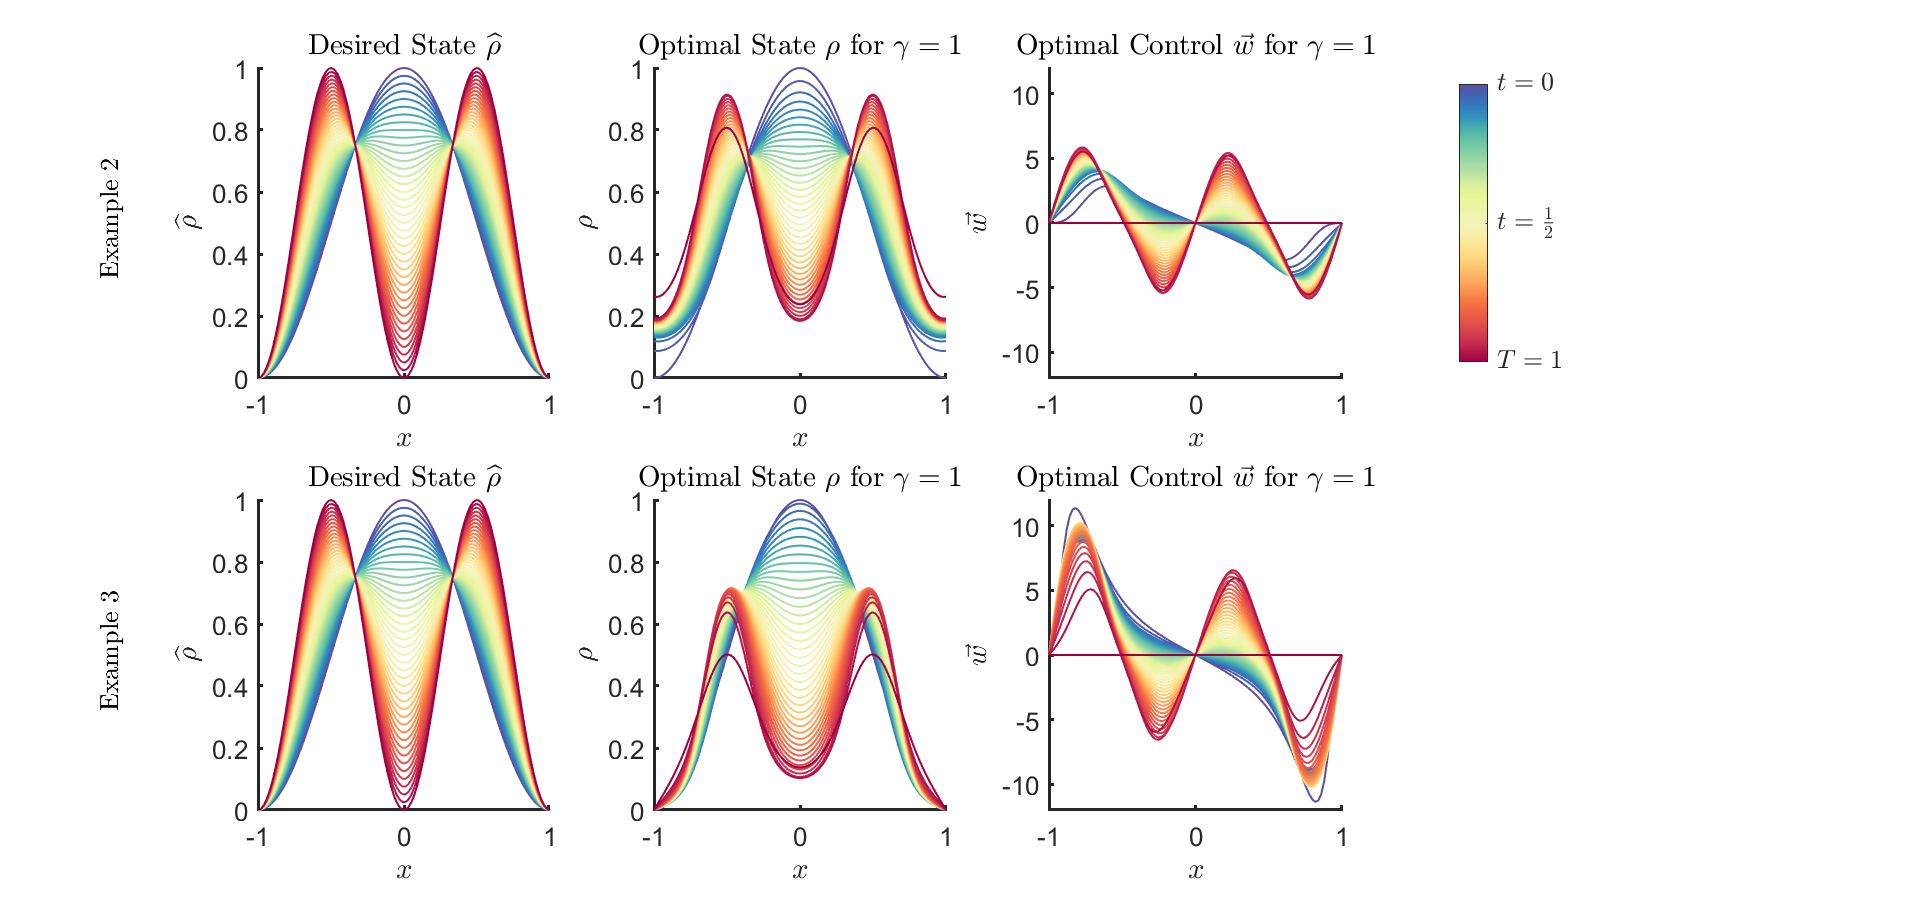
\includegraphics[scale=0.05]{Figure3.png}
	\caption{Example 2/ Example 3, desired state $\widehat \rho$, optimal state $\rho$ and corresponding optimal control $\vec{w}$, $\beta = 10^{-3}$, $\gamma = 1$.}
	\label{Ex22DN1}
\end{figure}

\begin{table}
\begin{tabular}{ | c | c || c | c | c | c ||}
\hline
\multicolumn{2}{|c||}{}& $\beta = 10^{-3}$ & $\beta = 10^{-1}$ & $\beta = 10^{1}$ & $\beta = 10^{3}$  \\
\hline
\hline
 & $\mathcal{J}_{uc}$ & $\numprint{0.0536}$ & $\numprint{0.0536}$ & $\numprint{0.0536}$ & $\numprint{0.0536}$ \\
$\kappa= \numprint{-1}$  & $\mathcal{J}_c$ & $\numprint{0.0096}$ & $\numprint{0.0492}$ & $\numprint{0.0535}$ & $\numprint{0.0536}$ \\
& \texttt{Iter} & $\numprint{715}$ & $\numprint{767}$ & $\numprint{367}$ & $\numprint{1}$ \\
\hline
 & $\mathcal{J}_{uc}$ & $\numprint{0.0669}$ & $\numprint{0.0669}$ & $\numprint{0.0669}$ & $\numprint{0.0669}$ \\
$\kappa= \numprint{0}$  & $\mathcal{J}_c$ & $\numprint{0.0109}$ & $\numprint{0.0603}$ & $\numprint{0.0668}$ & $\numprint{0.0669}$ \\
& \texttt{Iter} & $\numprint{714}$ & $\numprint{770}$ & $\numprint{390}$ & $\numprint{1}$ \\
\hline
 & $\mathcal{J}_{uc}$ & $\numprint{0.0839}$ & $\numprint{0.0839}$ & $\numprint{0.0839}$ & $\numprint{0.0839}$ \\
$\kappa= \numprint{1}$  & $\mathcal{J}_c$ & $\numprint{0.0125}$ & $\numprint{0.0748}$ & $\numprint{0.0838}$ & $\numprint{0.0839}$ \\
& \texttt{Iter} & $\numprint{713}$ & $\numprint{773}$ & $\numprint{403}$ & $\numprint{1}$ \\
\hline
\end{tabular}
\caption{Example 2: Cost when $\vec{w}=\vec{0}$, optimal control cost, and iterations required, for a range of $\kappa$, $\beta$.}
\label{TabS5:Prob2}
\end{table} %\label{TabS5:Prob2a}


\subsubsection{Dirichlet boundary conditions, Example 3} 
The inputs for this example are:
\begin{align*}
&\widehat \rho = \bigg(\frac{1}{2}\cos(\pi y) + \frac{1}{2}\bigg)(1-t) + t\bigg(-\frac{1}{2}\cos(2 \pi y) + \frac{1}{2}\bigg),\\
&\rho_{0} = \frac{1}{2}\cos(\pi y) + \frac{1}{2},\ \
\adj_{T} = 0,\ \
\vec{w} = \vec{0},\ \
f =0,\ \
V_{ext} =0.
\end{align*}
Table \ref{TabS5:Prob3} presents the results for this example, for a range of $\beta$ values and different interaction strengths. The observations are in line with those in Example 1 and 2. In particular, $ \widehat \rho$ and $\rho_0$ coincide with those of the problem with Neumann boundary conditions in Example 2. A comparison between the two examples is illustrated in Figure \ref{Ex22DN1}. Both the optimal state $\rho$ and the optimal control are qualitatively different when considering Dirichlet boundary conditions over Neumann conditions. The numerical result for this example was achieved with $N=40$ and $n = 30$, rather than with $N=30$ and $n=20$. This indicates that the Dirichlet boundary conditions are harder to apply in this problem, due to the steep shape of the desired state. This steepness is somewhat less impactful in Example 2, where the desired state is not closely matched by the optimal state at the boundaries. In Example 3, while the optimal state matches the desired state perfectly at the boundary, the peaks of the desired state are matched less closely. In Figure \ref{Ex22DN1}, this can be confirmed by considering the control plots. The optimal control for Example 3 is larger than for Example 2, specifically between the boundaries of the domain and the peaks of the desired state, indicating difficulties in this region.
\begin{table}
\begin{tabular}{ ||c|| c | c | c | c | c ||}
\hline
& & $\beta = 10^{-3}$ & $\beta = 10^{-1}$ & $\beta = 10^{1}$ & $\beta = 10^{3}$  \\
\hline
 & $J_{uc}$ & $\numprint{1.4165e-1}$ & $\numprint{1.4165e-1}$ & $\numprint{1.4165e-1}$ & $\numprint{1.4165e-1}$ \\
$\gamma= \numprint{-1}$  & $J_c$ & $\numprint{3.5594e-2}$ & $\numprint{1.3270e-1}$ & $\numprint{1.4155e-1}$ & $\numprint{1.4165e-1}$ \\
& $Iter.$ & $\numprint{944}$ & $\numprint{816}$ & $\numprint{437}$ & $\numprint{1}$ \\
\hline
 & $J_{uc}$ & $\numprint{1.5452e-1}$ & $\numprint{1.5452e-1}$ & $\numprint{1.5452e-1}$ & $\numprint{1.5452e-1}$ \\
$\gamma= \numprint{0}$  & $J_c$ & $\numprint{3.8023e-2}$ & $\numprint{1.4549e-1}$ & $\numprint{1.5442e-1}$ & $\numprint{1.5452e-1}$ \\
& $Iter.$ & $\numprint{940}$ & $\numprint{825}$ & $\numprint{440}$ & $\numprint{1}$ \\
\hline
 & $J_{uc}$ & $\numprint{1.6610e-1}$ & $\numprint{1.6610e-1}$ & $\numprint{1.6610e-1}$ & $\numprint{1.6610e-1}$ \\
$\gamma= \numprint{1}$  & $J_c$ & $\numprint{4.1143e-2}$ & $\numprint{1.5751e-1}$ & $\numprint{1.6601e-1}$ & $\numprint{1.6610e-1}$ \\
& $Iter.$ & $\numprint{932}$ & $\numprint{827}$ & $\numprint{440}$ & $\numprint{1}$ \\
\hline
\end{tabular}
\caption{Problem 3 ($n = 30,N = 40$)}
\label{TabS5:Prob3}
\end{table} %\label{TabS5:Prob3}


%\subsubsection{Neumann boundary conditions, Symmetric Example 1}
%Consider the following symmetric setup:
%\begin{align*}
%\widehat \rho &= \frac{1}{2}(1-t) + t\frac{1}{4}(\cos(\pi y)+2),\\
%\rho_{0} &= \frac{1}{2},\  \ q_{T} = 0, \ \ \vec{w} = \vec{0}, \ \  f =0, \ \ V_{ext} =0.
%\end{align*}
%Table \ref{TabNFlowAddEx1} summarizes the results for this example.The attractive interaction term causes $\rho$ to move towards the centre of the domain. Since $\widehat \rho$ is also centred in the domain, $J_{uc}$ is small for $\gamma =-1$ in comparison to the problems with $\gamma =0$ and $\gamma =1$. This example illustrates that the particle interaction term can have a significant impact on the optimization problem considered. 
%
%
%
%
%\subsubsection{Neumann boundary conditions, Symmetric Example 2}
%Consider the following symmetric setup, which is the opposite of the first symmetric example:
%\begin{align*}
%\widehat \rho &= \frac{1}{2}(1-t) + t\frac{1}{4}(-\cos(\pi y)+2),\\
%\rho_{0} &= \frac{1}{2},\ \
%q_{T} = 0,\ \
%\vec{w} = \vec{0},\ \
%f =0,\ \
%V_{ext} =0.
%\end{align*}
%This example can be compared to the Symmetric Example 1. Here, the desired state is having $\rho$ clustered at both boundaries, which is similar to the effect of the repulsive interaction term $\gamma = 1$. Therefore, for this choice of interaction term, the value of the cost functional $J_{uc}$ is smaller than the one for $\gamma = 0$ and $\gamma = -1$. This is the opposite to the observation made in the Symmetric Example 1, which is to be expected, given the two choices of desired state.


\subsection{Linear control problems with an additional nonlocal integral term}
In this section, examples of solving Problem \eqref{AdvDiff_Linear} with both 'no-flux type' boundary conditions \eqref{NoFlux_Linear} and Dirichlet boundary conditions \eqref{Dirichlet}.
\subsubsection{Dirichlet boundary conditions, Example 4}
The inputs for this example are:
\begin{align*}
&\widehat \rho = (1 - t)\bigg(\frac{1}{2}\cos(\pi y) + \frac{1}{2}\bigg)  + t\bigg(-\frac{1}{2}\cos(\pi y) + \frac{1}{2}\bigg),\\
&\rho_{0} = \frac{1}{2}\cos(\pi y) + \frac{1}{2},\ \
\adj_{T} = 0,\ \
{w} = 0,\ \
f =0, \ \
V_{ext} =\frac{1}{2}\left((x + 0.3)^2 - 0.2\right)\left((x-0.4)^2 - 0.3\right).
\end{align*}
In Table \ref{TabS5:Prob4} the results for Example 4 for a range of parameter values can be found. The results are qualitatively similar to the previous examples, but the control is applied linearly in this example. Note that here $\lambda = 0.005$, since $V_{{ext}}$ causes the numerical computations to be more challenging.
\begin{table}
\begin{tabular}{ | c | c || c | c | c | c ||}
\hline
\multicolumn{2}{|c||}{}& $\beta = 10^{-3}$ & $\beta = 10^{-1}$ & $\beta = 10^{1}$ & $\beta = 10^{3}$  \\
\hline
\hline
 & $\mathcal{J}_{uc}$ & $\numprint{0.1394}$ & $\numprint{0.1394}$ & $\numprint{0.1394}$ & $\numprint{0.1394}$ \\
$\kappa= \numprint{-1}$  & $\mathcal{J}_c$ & $\numprint{0.0183}$ & $\numprint{0.0862}$ & $\numprint{0.1384}$ & $\numprint{0.1394}$ \\
& \texttt{Iter} & $\numprint{1575}$ & $\numprint{1486}$ & $\numprint{1026}$ & $\numprint{117}$ \\
\hline
 & $\mathcal{J}_{uc}$ & $\numprint{0.1526}$ & $\numprint{0.1526}$ & $\numprint{0.1526}$ & $\numprint{0.1526}$ \\
$\kappa= \numprint{0}$  & $\mathcal{J}_c$ & $\numprint{0.0183}$ & $\numprint{0.0983}$ & $\numprint{0.1516}$ & $\numprint{0.1526}$ \\
& \texttt{Iter} & $\numprint{1582}$ & $\numprint{1474}$ & $\numprint{1023}$ & $\numprint{113}$ \\
\hline
 & $\mathcal{J}_{uc}$ & $\numprint{0.1645}$ & $\numprint{0.1645}$ & $\numprint{0.1645}$ & $\numprint{0.1645}$ \\
$\kappa= \numprint{1}$  & $\mathcal{J}_c$ & $\numprint{0.0189}$ & $\numprint{0.1103}$ & $\numprint{0.1635}$ & $\numprint{0.1645}$ \\
& \texttt{Iter} & $\numprint{1589}$ & $\numprint{1465}$ & $\numprint{1022}$ & $\numprint{112}$ \\
\hline
\end{tabular}
\caption{Example 4: Uncontrolled cost $\mathcal{J}_{uc}$, optimal cost $\mathcal{J}_{c}$, and number of iterations, for a range of $\kappa$ and $\beta$ values.}
\label{TabS5:Prob4}
\end{table} %\label{TabS5:Prob4}




\subsubsection{Neumann boundary conditions, Example 5}
The inputs for this example are:
\begin{align*}
&\widehat \rho = \frac{1}{2}(1-t) + t\frac{1}{2}(-\cos(\pi y) + 1),\\
&\rho_{0} = \frac{1}{2},\ \
\adj_{T} = 0,\ \
{w} = 0,\ \
f =0,\ \
V_{ext} =0.
\end{align*}
Table \ref{TabS5:Prob5} shows the results for Example 5. Note that for this example, when $\beta = 10^{-3}$, the mixing parameter $\lambda$ had to be set to $0.001$, to guarantee stable convergence of the method (why? explanation needed?).
Again, the only qualitative difference to interpreting the results is that the control is applied linearly.
\begin{table}
\begin{tabular}{ ||c|| c | c | c | c | c ||}
\hline
& & $\beta = 10^{-3}$ & $\beta = 10^{-1}$ & $\beta = 10^{1}$ & $\beta = 10^{3}$  \\
\hline
 & $J_{uc}$ & $\numprint{6.0640e-2}$ & $\numprint{6.0640e-2}$ & $\numprint{6.0640e-2}$ & $\numprint{6.0640e-2}$ \\
$\gamma= \numprint{-1}$  & $J_c$ & $\numprint{6.0180e-3}$ & $\numprint{5.5365e-2}$ & $\numprint{6.0592e-2}$ & $\numprint{6.0640e-2}$ \\
& $Iter.$ & $\numprint{7320}$ & $\numprint{7712}$ & $\numprint{3888}$ & $\numprint{1}$ \\
\hline
 & $J_{uc}$ & $\numprint{4.1667e-2}$ & $\numprint{4.1667e-2}$ & $\numprint{4.1667e-2}$ & $\numprint{4.1667e-2}$ \\
$\gamma= \numprint{0}$  & $J_c$ & $\numprint{4.5414e-3}$ & $\numprint{3.8334e-2}$ & $\numprint{4.1632e-2}$ & $\numprint{4.1667e-2}$ \\
& $Iter.$ & $\numprint{7271}$ & $\numprint{7614}$ & $\numprint{3643}$ & $\numprint{1}$ \\
\hline
 & $J_{uc}$ & $\numprint{2.8551e-2}$ & $\numprint{2.8551e-2}$ & $\numprint{2.8551e-2}$ & $\numprint{2.8551e-2}$ \\
$\gamma= \numprint{1}$  & $J_c$ & $\numprint{3.5942e-3}$ & $\numprint{2.6480e-2}$ & $\numprint{2.8529e-2}$ & $\numprint{2.8551e-2}$ \\
& $Iter.$ & $\numprint{7249}$ & $\numprint{7482}$ & $\numprint{3410}$ & $\numprint{1}$ \\
\hline
\end{tabular}
\caption{Problem 5}
\label{TabS5:Prob5}
\end{table} %\label{TabS5:Prob5}


\subsection{Nonlinear control problems with an additional nonlocal integral term in 2D}
In this section, two-dimensional examples are considered, to illustrate the fact that the application of the method differs very little from the one dimensional setting. The main difference is that in nonlinear control problems the control is a two-dimensional vector field. Furthermore, the number of spatial points increases from $N$ to $N_1\times N_2$, which makes computations much more costly. Compensating for this increased cost is one of the motivations to develop fast optimization solvers, such as the fixed point method introduced in Section \ref{sec:Method_Solver}.
\subsubsection{Neumann boundary conditions, Example 1}	
We have the following set up:
\begin{align*}
&\widehat \rho = \frac{1}{4}(1-t) + t\bigg(\frac{1}{4}\sin \bigg(\frac{\pi}{2}(x_1 - 2)\bigg)\sin \bigg(\frac{\pi}{2}(x_2 - 2)\bigg) + \frac{1}{4}\bigg),\\
&\rho_0 = \frac{1}{4},\ \
q_{T} = 0,\ \
\vec{w} = \vec{0},\ \
f =0,\ \
V_{ext} =0.
\end{align*}
This example is the two dimensional version of Example 1 in Section \ref{sec:Examples1d}. The results for this example are displayed in Table \ref{TabS5:Prob12D}. In Figures \ref{rhoHat2dEx2} it can be observed that as in Example 1 in Section \ref{sec:Examples1d}, the uncontrolled state forms a cluster in the centre of the domain, due to the attractive interactions. Figure \ref{rhoOpt2dEx2} shows the optimal state and control for different time points, for $\beta = 10^{-3}$ and $\gamma = -1$. Here, the control through a vector field illustrates why nonlinear control is called 'flow control'. 

\begin{table}
\begin{tabular}{ ||c|| c | c | c | c | c ||}
\hline
& & $\beta = 10^{-3}$ & $\beta = 10^{-1}$ & $\beta = 10^{1}$ & $\beta = 10^{3}$  \\
\hline
 & $\mathcal J_{\vec w = \vec 0}$ & $0.0113$ & $0.0113$ & $0.0113$ & $0.0113$ \\
$\kappa= -1$  & $\mathcal J_{Opt}$ & $0.0013$ & $0.0104$ & $0.0113$ & $0.0113$ \\
& $\text{Iterations}$ & $676$ & $700$ & $290$ & $1$ \\
\hline
\end{tabular}
\caption{Results for the test problem, with different $\beta$}
\label{TabS5:Prob12D}
\end{table} % \label{TabS5:Prob12D}

\begin{figure}[h]
	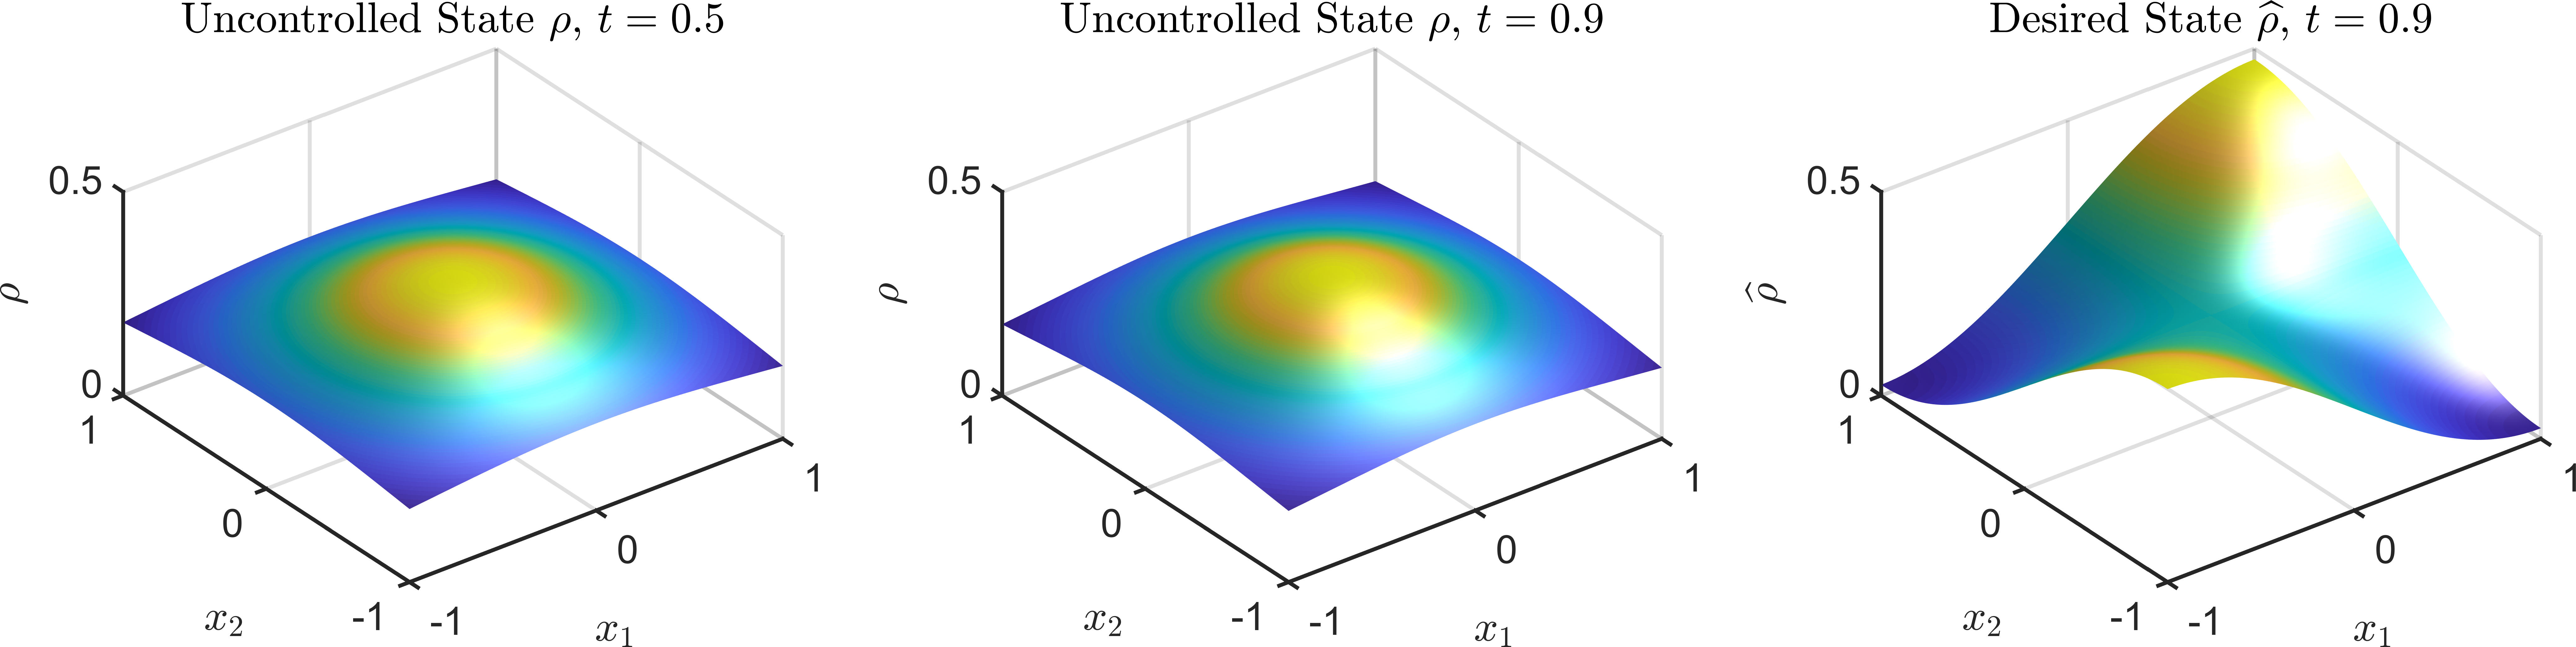
\includegraphics[scale=0.05]{Figure12D.png}
	\caption{2D Example 1, uncontrolled $\rho$ and $\widehat \rho$, $\beta = 10^{-3}$, $\gamma = -1$.}
	\label{rhoHat2dEx2}
\end{figure}
\begin{figure}[h]
	\includegraphics[scale=0.06]{Figure22D.png}
	\caption{2D Example 1, controlled $\rho$ and optimal control $\vec{w}$, $\beta = 10^{-3}$, $\gamma = -1$.}
	\label{rhoOpt2dEx2}
\end{figure}


\subsubsection{Neumann boundary conditions, Example 2}	
Here, we have:
\begin{align*}
&\widehat \rho = \frac{1}{4}(1-t) + t\frac{1}{0.9921}e^{-3((y_1+0.2)^2 + (y_2+0.2)^2))},\\
&\rho_0 = \frac{1}{4},\ \
q_{T} = 0,\ \
\vec{w} = \vec{0},\ \
f =0,\\
&V_{ext} =\left((x_1 + 0.3)^2 - 1\right)\left((x_1-0.4)^2 - 0.5\right)
\left((x_2 + 0.3)^2 - 1\right)\left((x_2-0.4)^2 - 0.5\right).
\end{align*}
The numerical results for this example are displayed in Table \ref{TabS5:Prob22D}. In figures \ref{rhoHat2dEx4} and \ref{rhoOpt2dEx4} the results are illustrated for $\beta = 10^{-3}$ and $\gamma = -1$. It can be observed very clearly that the control is driving the particle distribution to the desired state. It is noticeable that the control does not act uniformly around the peak of the desired state, but also acts strongly in the area between the location of the desired peak and the point $(-1,1)$. This is due to the external potential being steep in this area and more control is needed to reach the desired state than in other parts of the domain.

\begin{table}
\begin{tabular}{ | c | c || c | c | c | c ||}
\hline
\multicolumn{2}{|c||}{}& $\beta = 10^{-3}$ & $\beta = 10^{-1}$ & $\beta = 10^{1}$ & $\beta = 10^{3}$  \\
\hline
\hline
 & $\mathcal{J}_{uc}$ & $\numprint{0.0378}$ & $\numprint{0.0378}$ & $\numprint{0.0378}$ & $\numprint{0.0378}$ \\
$\kappa= \numprint{-1}$  & $\mathcal{J}_c$ & $\numprint{0.0017}$ & $\numprint{0.0312}$ & $\numprint{0.0377}$ & $\numprint{0.0378}$ \\
& \texttt{Iter} & $\numprint{691}$ & $\numprint{736}$ & $\numprint{347}$ & $\numprint{1}$ \\
\hline
 & $\mathcal{J}_{uc}$ & $\numprint{0.0478}$ & $\numprint{0.0478}$ & $\numprint{0.0478}$ & $\numprint{0.0478}$ \\
$\kappa= \numprint{0}$  & $\mathcal{J}_c$ & $\numprint{0.0064}$ & $\numprint{0.0450}$ & $\numprint{0.0478}$ & $\numprint{0.0478}$ \\
& \texttt{Iter} & $\numprint{718}$ & $\numprint{784}$ & $\numprint{343}$ & $\numprint{1}$ \\
\hline
 & $\mathcal{J}_{uc}$ & $\numprint{0.0526}$ & $\numprint{0.0526}$ & $\numprint{0.0526}$ & $\numprint{0.0526}$ \\
$\kappa= \numprint{1}$  & $\mathcal{J}_c$ & $\numprint{0.0137}$ & $\numprint{0.0514}$ & $\numprint{0.0526}$ & $\numprint{0.0526}$ \\
& \texttt{Iter} & $\numprint{735}$ & $\numprint{790}$ & $\numprint{338}$ & $\numprint{1}$ \\
\hline
\end{tabular}
\caption{2D Ex. 2: Uncontrolled cost $\mathcal{J}_{uc}$, optimal cost $\mathcal{J}_{c}$, and number of iterations, for a range of $\kappa$ and $\beta$ values.}
\label{TabS5:Prob22D}
\end{table} %\label{TabS5:Prob22D}

\begin{figure}[h]
	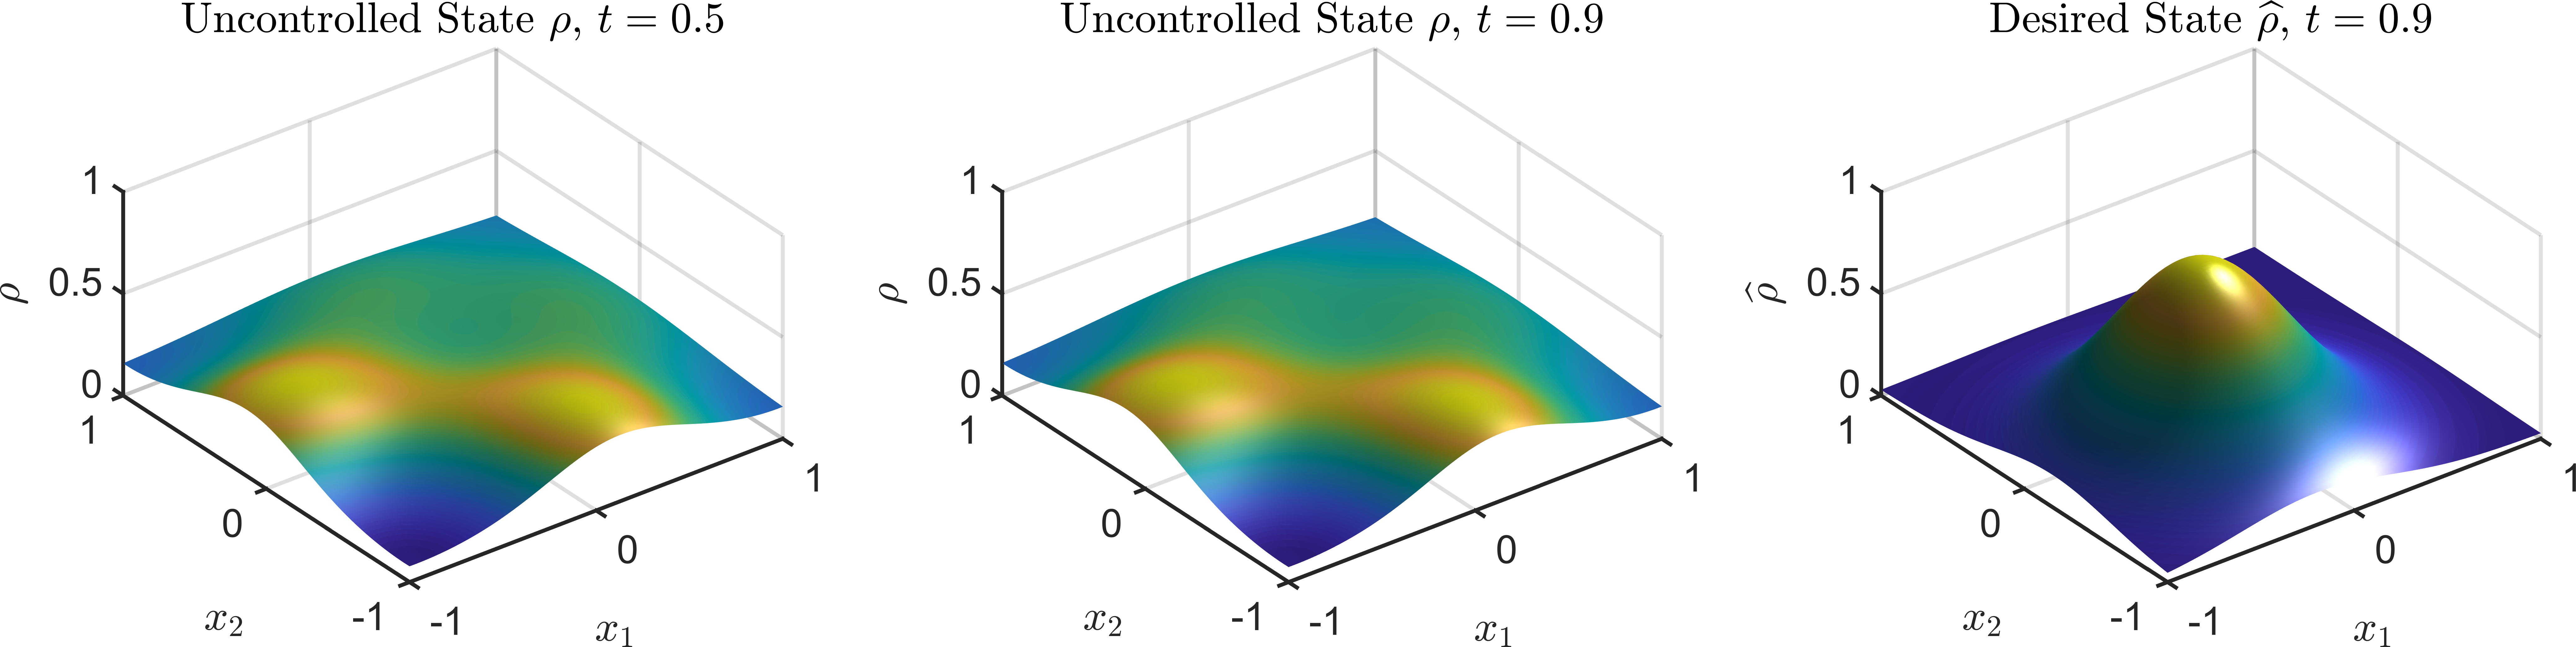
\includegraphics[scale=0.05]{Figure32D.png}
	\caption{2D Example 2: Uncontrolled $\rho$ and desired state $\widehat \rho$,  with $\beta = 10^{-3}$ and $\kappa = -1$. }
	\label{rhoHat2dEx4}
\end{figure}
\begin{figure}[h]
	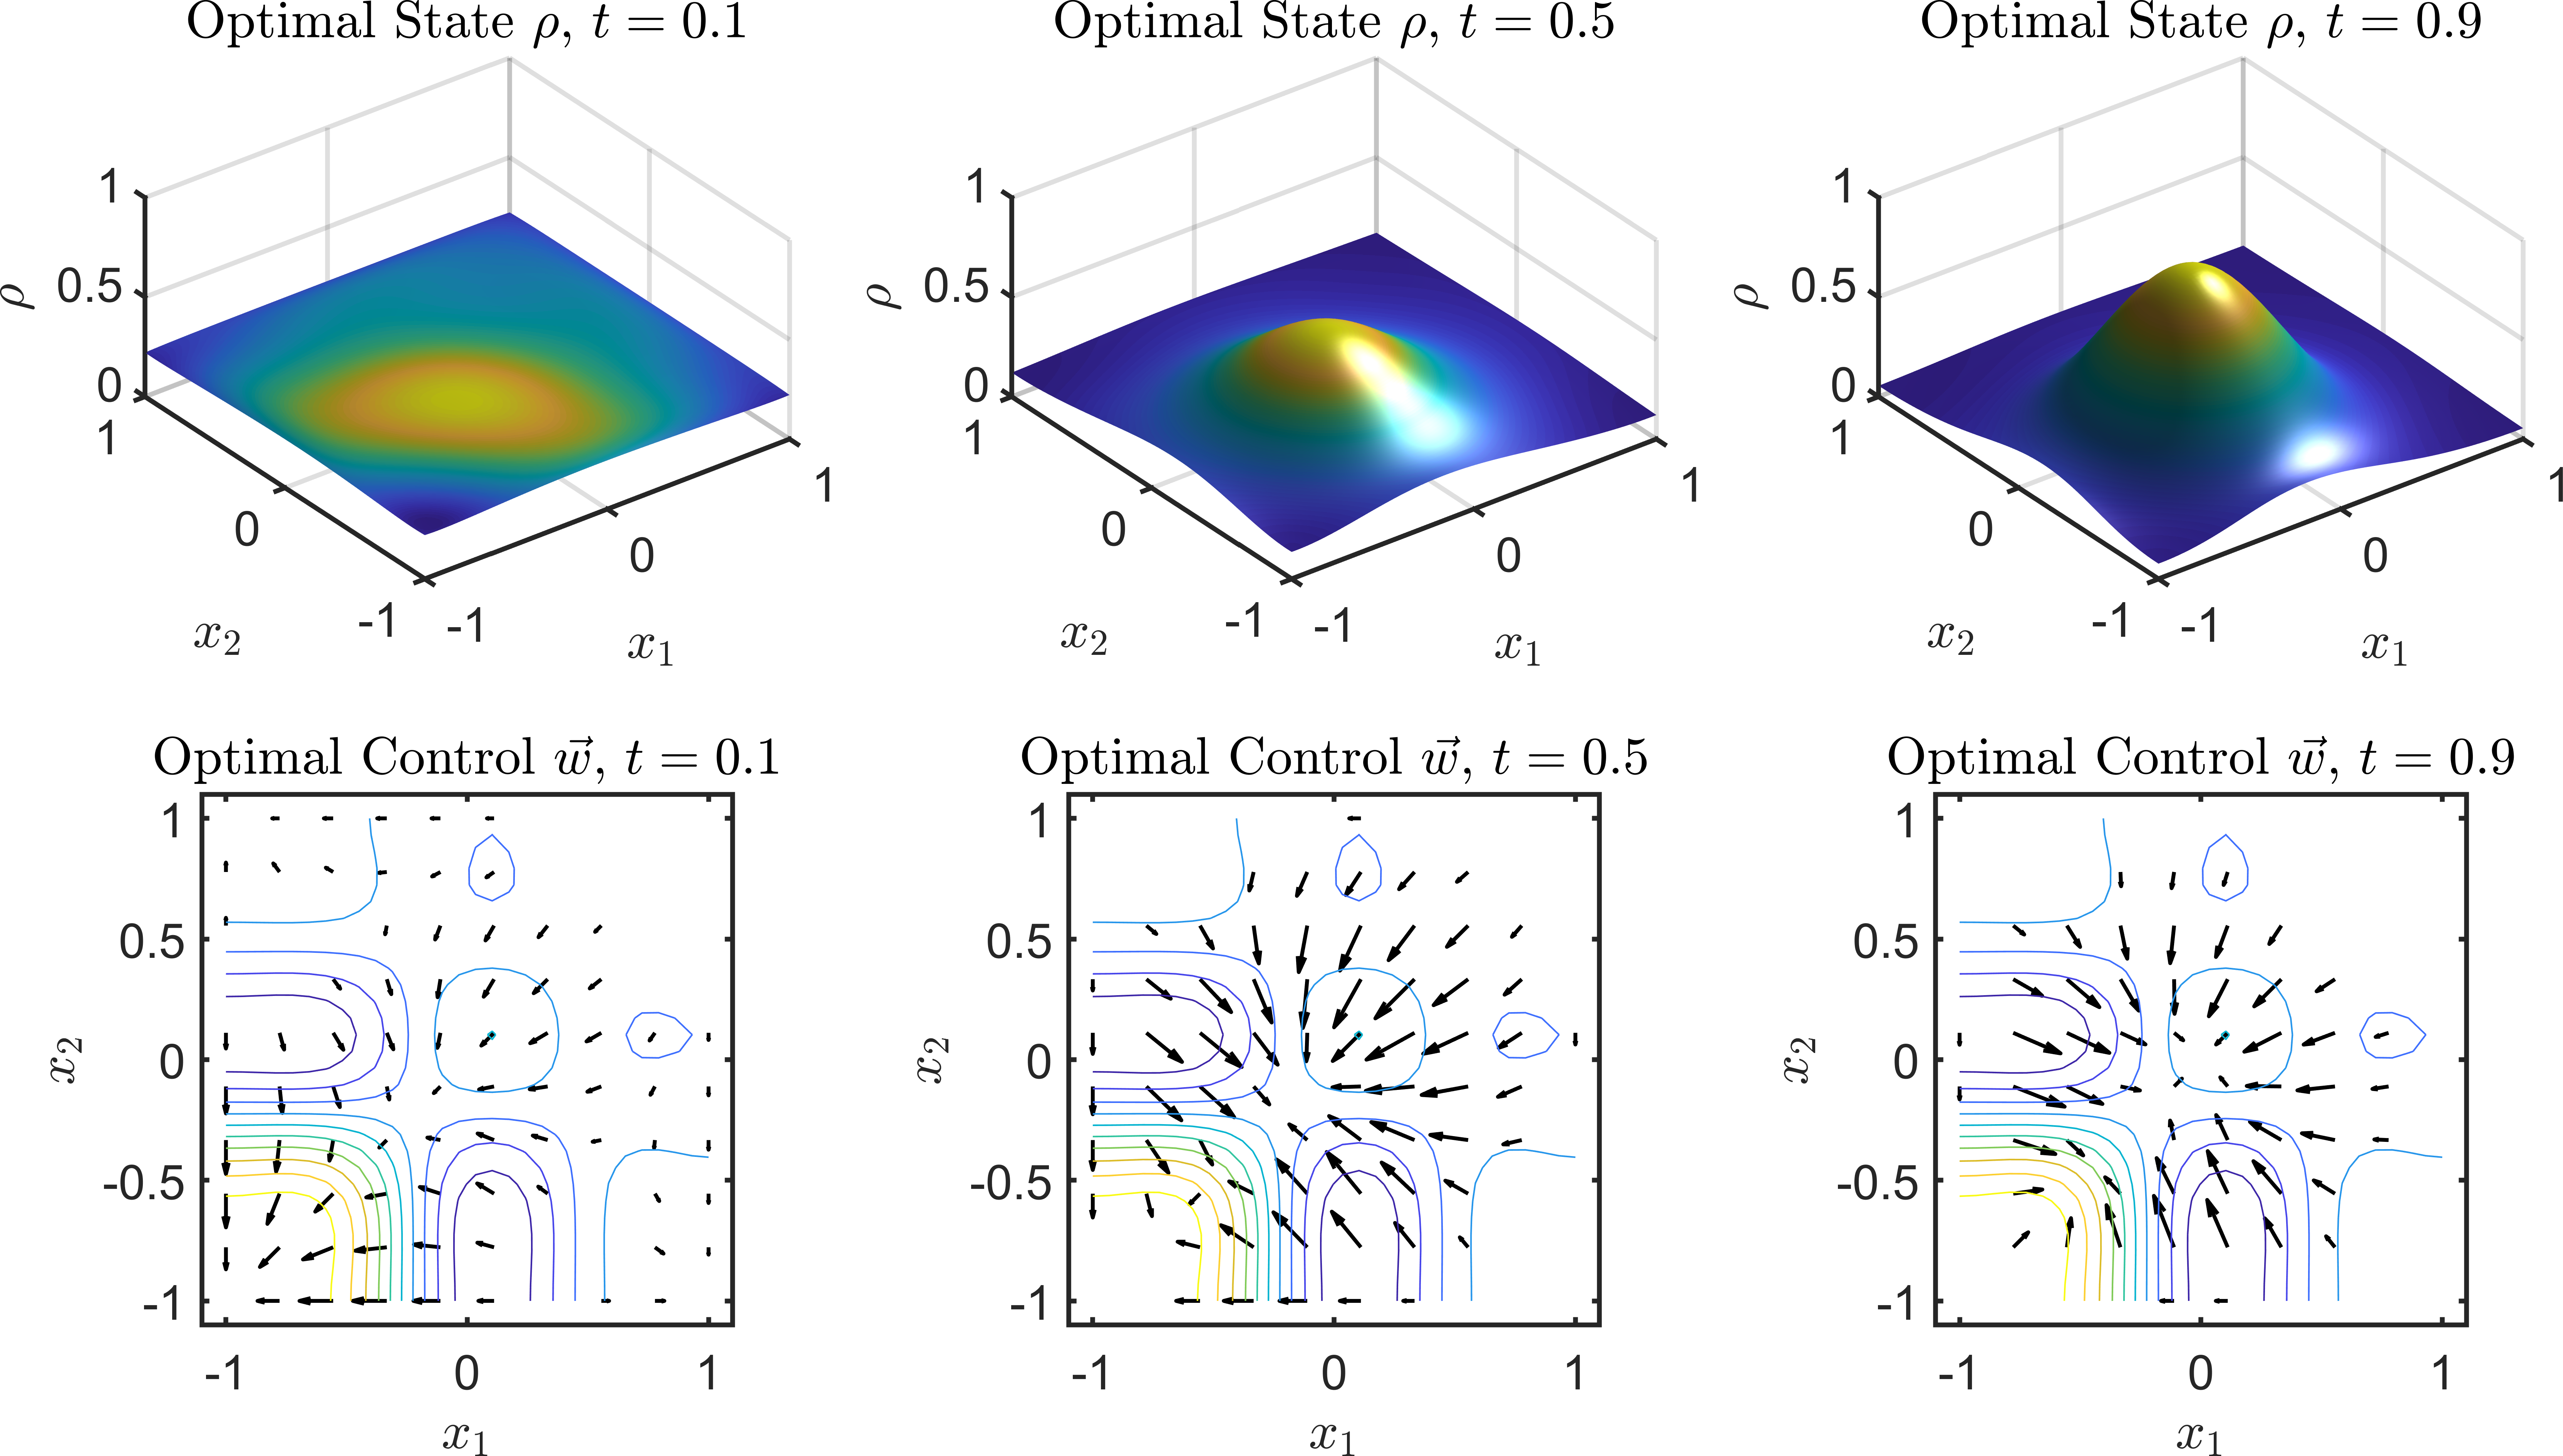
\includegraphics[scale=0.06]{Figure42D.png}
	\caption{2D Example 2: Optimal state $\rho$ and optimal control $\vec{w}$, with $\beta = 10^{-3}$ and $\kappa = -1$. A contour plot of the external potential $V^{\text{ext}}$ is superimposed on the control plots for reference.} 
	\label{rhoOpt2dEx4}
\end{figure}









\section{Conclusion}
During the past year a fast and accurate optimization solver has been developed, which reliably solves various optimal control problems. In the course of the next year, this will be applied to different problems. For example, inertial effects will be included in the optimal control problem. Furthermore, the numerical method is extended to be applied to different domains. At the present time, only rectangular domains are considered. However, in the following year, the optimal control problems will be solved on more complex domains, which are composed of quadrilateral and circular shapes. 
Other possible extensions to be considered are models including multiple species and different control types other than flow and source control.
The main aim is to enable the application of the model and numerical method to industrial applications.


\pagebreak	
\bibliography{GeneralBib}
\bibliographystyle{unsrt}

\pagebreak
\appendix

\section{Activities Besides the PhD Project}
\subsection{Teaching}
I have been teaching four courses over the past two semesters. These include 'Introduction to Linear Algebra' (Y1), 'Several Variable Calculus and Differential Equations' (Y2), 'Honours Algebra (Skills)' (Y3) and 'Honours Complex Variables' (Y3).\\
The first and second year classes were in small workshop groups, 'Honours Algebra (Skills)' was taught in a computer lab and focussed on the algebra software 'Sage'. 'Honours Complex Variables' was an open tutorial with half of the student cohort and several tutors in the same room at each session.\\
Furthermore, I participated in the markfests for 'Introduction to Linear Algebra' and 'Several Variable Calculus and Differential Equations'. I have also marked a question (remotely due to Covid-19) for the 'Honours Complex Variables' final exam.
\subsection{Classes and Autumn School}
In the first semester of this year, I have attended the MSc course on Stochastic Analysis, a mini-course on Industrial Mathematics and an Autumn School on Optimal Control and Optimization with PDEs. In the second semester I have taken the advanced MIGSAA course on Numerical Analysis of Partial Differential Equations. In total I have been awarded 45 credits.
\subsection{Generic Skills}
I have completed seven generic skills activities this year, as stated in the logbook. I have been a co-organiser of the MIGSAA Annual Colloquium in September 2019. I have taken two semesters of Spanish classes via the University's short courses. Furthermore, I have been a Mentor for the MAC-MIGs students. I have organised the PG Colloquium for the past two semesters, and, collaboratively with Heriot-Watt, organised an online PhD seminar during the summer, the Maxwell PhD Seminar.
Lastly, I got two generic skills credits for the tutoring and marking activities mentioned in the teaching section above.
\subsection{Citizenship}
I have attended most ACM seminars this year, some analysis and optimization seminars in UoE and some mathematical biology meetings in HW. I have also attended most of the sessions of the MAC-MIGs Modelling course. I have, as organiser, attended all but one PG Colloquium sessions, as well as all Maxwell PhD Seminar sessions.
I have given a talk at the SIAM-IMA Student Chapter PhD Colloquium, presented a poster at the Annual MIGSAA Colloquium, and presented my work at a 'This is what we do' session to the MAC-MIGs students. I was supposed to give a talk about my work at the BAMC in Glasgow in April, which has been postponed to 2021 due to the current situation. I have given a talk at the LMS Scottish Numerical Methods Network workshop on Multiscale Methods in June. In terms of outreach work, I have held a 10 minute talk about PhD life to Y4 and Y5 undergraduate UoE students and I co-facilitated a lunch meeting, organised by the Piscopia Initiative, aimed at female undergraduate students in order to enhance postgraduate applications from female students. While this type of event was organised for different Schottish universities, the one I attended has been at the University of Glasgow.
Finally, as the organiser of the PG Colloquium I have also been an active part in the UoE PG Committee, such as by helping to organise the departmental christmas party. Currently we are preparing strategies on how to welcome the new PhD cohort in Edinburgh, as well as working on offering different social activities for the existing PhD community to decrease impact of Covid-19 measures on the social life of all PhD students.

\subsection{Outlook}
Outside my research project I am planning to get involved in the following activities during the next year.
I will take at least one more class for credits. I may attend a second class for credits or attendance only, depending on my other commitments. In terms of knowledge enhancement, I would like to focus on catching up on PDE Theory/Analysis, as well as on expanding my coding skills, by learning Python or a similar language. ++ maybe more optimization techniques too -- goes with career stuff\\
I hope to increase my involvement in conferences and workshops, sharing my work by giving talks, presenting posters and networking with different people. I will continue to attend seminars and workshops on different topics. I am hoping that, additionally, I will take part in an academic/ industry focussed study group.\\
I want to invest some of my additional time in career planning and skills development. This can mean taking workshops, coding classes or by seeking out networking opportunities.\\ 	
I am now a member of the SIAM-IMA Student Chapter Committee in Edinburgh and we are planning to host a series of events with different focus, such as outreach, industry, social events and PhD research talks. 
I also hope to be involved with some projects of the Piscopia Initiative as well as with the PG Committee in a more casual function. \\




\end{document}